\documentclass[preprint,nocopyrightspace,10pt]{sigplanconf}
%\documentclass[9pt]{sigplanconf}
%\documentclass{sigplanconf}

% The following \documentclass options may be useful:
%
% 10pt          To set in 10-point type instead of 9-point.
% 11pt          To set in 11-point type instead of 9-point.
% authoryear    To obtain author/year citation style instead of numeric.

\usepackage{amsmath}
\usepackage{graphicx}
\usepackage{graphics}
\usepackage{comment}
\usepackage{amsmath}
\usepackage{algorithm}
\usepackage{algpseudocode}
\usepackage{color}
\usepackage{subfig}
\usepackage{multirow}
\usepackage[normalem]{ulem}
\usepackage{amsthm}
\usepackage{mathtools}

\newcommand{\asplossubmissionnumber}{228}
\renewcommand{\algorithmicrequire}{\textbf{Globals:}}
\renewcommand{\algorithmicensure}{\textbf{Output:}}

\newtheorem{defn}{Definition}
\newtheorem{theorem}{Theorem}[section]
\newtheorem{property}{Property}[section]
\newtheorem{corollary}{Corollary}[theorem]
\newtheorem{lemma}[theorem]{Lemma}

\begin{document}

\title{Optimizing Data Persistence: A Software Cache Approach}
%\subtitle{Subtitle Text, if any}

\authorinfo{}{}{}


%\date{}
\maketitle

\begin{abstract}

Persistent memory is getting increasingly popular because it enables reuse of data in
memory regardless of failures. However, the existence of transient CPU caches in
modern computer architectures brings a serious performance issue for utilization of
persistence. In particular, cache lines have to be flushed frequently to guarantee
consistent, persistent program states. Hence, persistence and performance cannot
be easily obtained simultaneously.

In this paper, we optimize data persistence by proposing a software cache solution. 
The software cache first buffers lines that need to be flushed, and then flushes them 
out at appropriate later time. The software cache aims to maximize the overlap of cache
line flushes. We designed a new linear-time algorithm to calculate cache miss ratio
curve (MRC) so as to adaptively select the best cache capacity at runtime based on
program behavior. We designed an expiration list to maximally hide the cost of memory
transfer of cache lines. We evaluated the software cache solution on four
micro-benchmarks, the SPLASH2 benchmark suite and a real-world in-memory database
application. Results turn out that the software cache solution significantly reduce
cache line flushes by $183\times$ and improves performance over 
the state-of-the-art by $1.4\times$ on average.

\end{abstract}

\section{Introduction}
\label{sec:intro}

Persistent memory or non-volatile memory (NVRAM) technologies, such as memristors~\cite{Memristor:2008}
and phase change memory (PCM)~\cite{Qureshi:ISCA09,Lee:ISCA09}, are getting increasingly popular. Intel
just announced that its non-volatile memory technology, 3D XPoint~\cite{3DXPoint:2014},
will be productized in the near future. Persistent memory offers high density, low power,
and fast access latency that is comparable to that of DRAM. 

Persistent memory is byte-addressable and directly accessible (i.e. without DRAM buffers)
with CPU loads and stores. The direct access helps reduce latency of
the middleware layers if they take advantage of NVRAM. Data in NVRAM
will not be erased if the creating process doesn't  
clean it. It enables data reuse across system restarts and of course process restarts.
This in-memory durability model~\cite{Dhruva+:OOPSLA14} can greatly
change programming paradigm for some 
applications. While an application today typically maintains an
in-memory object format and a separate durable format for a durable
block device, only one format of data will suffice in this new world. 
As a result, program structure and code maintenance are vastly
improved. 

However, nothing comes for free. Though NVRAM enables simpler data reuse,
data consistency and runtime performance challenges remain. 
To reuse, applications ought to preserve consistent intermediate
states. However, transient memories in current computer architectures,
such as CPU caches, pose a performance challenge for this
requirement. As described in ~\cite{Dhruva+:OOPSLA14}, at any point of
program execution, some of the updates to persistent memory may only
reside in CPU caches because they have not yet propagated to NVRAM. If
there is a failure at this point of execution, the program state in
NVRAM may not be consistent thus preventing its reuse. The solution is
to flush out dirty cache lines at appropriate program points so that
the above situation cannot occur. 

% DC: This example is almost directly lifted out of the Atlas
% paper. Instead of providing such a similar example, I think it is
% better to just cite the paper and explain in abstract terms. here is
% my attempt at it.

%\begin{figure}[hbpt]
%   \centering
%   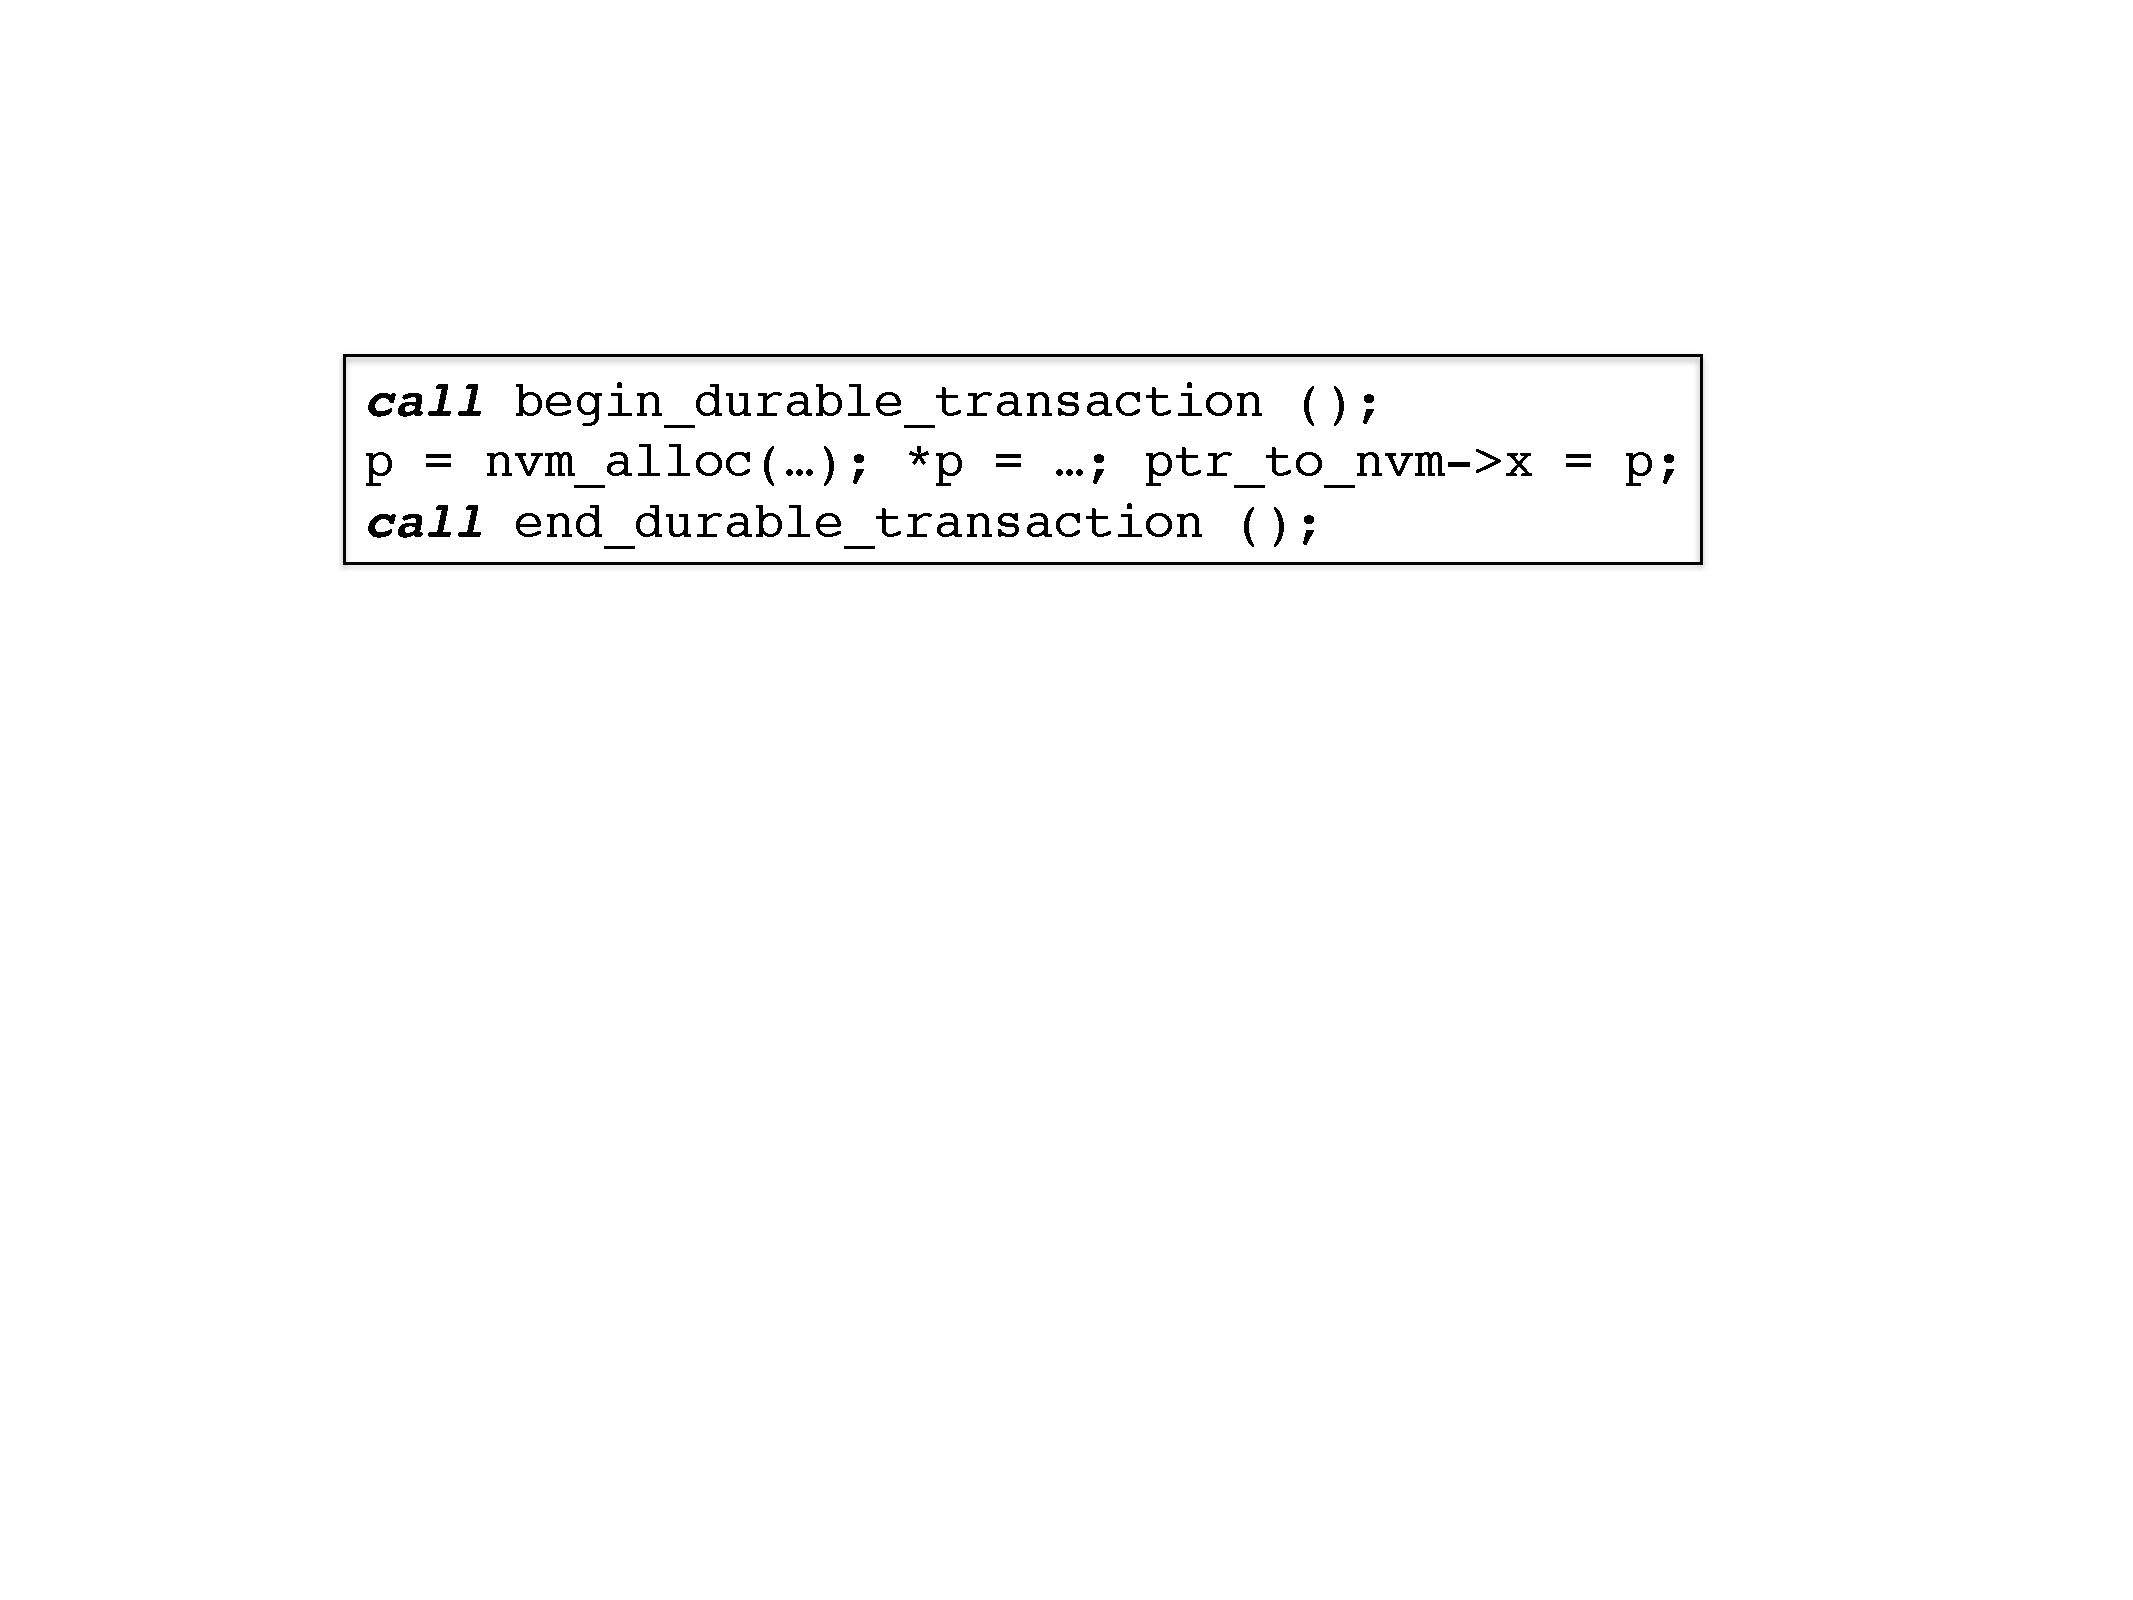
\includegraphics[width=0.45\textwidth]{./figures/code.pdf}
%   \caption{Allocation, initialization and publication.}
%   \label{fig:code}
%\end{figure}

%Let's consider the code example in Figure~\ref{fig:code}. It shows that a persistent memory
%region $p$ is allocated, initialized, and then published, by assigning it a persistent field $x$, within
%a so-called durable transaction. The durable transaction means after its execution,
%data in persistent memory must appear to be consistent. Due to the
%existence of CPU caches,  
%the store to the persistent location $p$ ($*p = ...$) may have not yet been written back
%after the durable transaction and before a follow-up machine crash.  When the program 
%restarts and resumes after the durable transaction, it has a stale value for the persistent 
%location, meaning a inconsistent state and hence non-reusable. 
%
%To make it consistent, at the end of the durable transaction, the cache line of the specific store 
%requires to be flushed out. In Figure~\ref{fig:code}, the cache lines of $p$ and $\&x$ both
%need to be flushed out. 

Consequently, a substantial amount of cache line flushes are involved to maintain consistent
durability. A naive approach is to flush every store immediately, as it finishes, from cache
to persistent memory. However, its performance loss is unacceptable. We measured this
approach for SPLASH2~\cite{Woo+:ISCA95} benchmark. Performance drops by 22$\times$ on average,
as shown in Table~\ref{tbl:moti}. This paper addresses performance
optimizations of cache line flushes. 

\begin{table}[hbpt]
\small
\centering
\begin{tabular}{c|c|c|c}
\hline
{\bf Program} & {\bf Slowdown} & {\bf Program}& {\bf Slowdown}  \\ \hline
barnes & 22$\times$ & fmm & 24$\times$ \\ \hline
ocean & 17$\times$ & raytrace & 6$\times$  \\ \hline
volrend & 26$\times$ & water-nsquared & 24$\times$ \\ \hline
water-spatial & 33$\times$ & {\bf average} & 22$\times$  \\\hline
\end{tabular}
\caption{The worst-case time cost to persist data.}
\label{tbl:moti}
\end{table}

% TODO DC: Revisit the following paras in this section.
In this paper, we propose a software cache approach to optimize cache
line flushes. For every persistent memory store, we buffer its cache
line in the software cache and try to overlap the flushes of the same
cache line. We propose a new metric, called \emph{all-window reuse},
and a linear-time algorithm around it to compute the \emph{miss ratio
curve} (MRC) for a given application, based on which cache capacity is
selected.  Flushing too many cache lines at a time at the end of a
durable transaction stalls CPU for a long time. To alleviate this
problem, we propose \emph{the expiration list} to flush unused cache
lines in advance.

Specifically, we make the following contributions:
\begin{itemize}
\item We proposed a software cache approach to optimize cache line
flushes;
\item We proposed a new metric, called \emph{all-window reuse}. It is
a higher order than cache hit ratio. It complements a recent cache
locality theory~\cite{Xiang+:ASPLOS13} from another angle;
\item We developed a new linear-time algorithm to compute
\emph{all-window reuse} and hence MRC. We use MRC to select the best
cache capacity.
\item We designed the software cache in $O(1)$ time; 
\item We evaluated the software cache approach on 13 programs,
including 4 micro-benchmarks, SPLASH2 benchmark suite and a in-memory
database application, and compared with four other approaches. Results
turn out that the software cache approach significantly reduces cache
line flushes by 183$\times$ and improves performance over the
state-of-the-art by 1.4$\times$ for one thread run.
\end{itemize}

\section{Preliminaries}
\label{sec:back}
Current computer memory hierarchy takes advantage of volatile memory, such as
cache, volatile buffers and DRAM, for the sake of speed, even in the presence of 
NVRAM. The co-existence of volatile memory and NVRAM may incur inconsistent 
persistence states. For example, a machine crashes when part of data is in cache 
and the rest is in NVRAM. The persistent data cannot be reused if inconsistent 
persistence states exist.

Consistent persistence states are guaranteed by writing back all data from volatile
memory to persistent memory in the event of any tolerated failure. 
It is unacceptable to conjecture which machine failure or when to fail is tolerated, therefore
users partition a program execution into many durable transactions and at the end of a
durable transaction, data is written back to persistent memory. An end of a transaction
foresees a machine failure. Consistent persistence is always guaranteed at the end of 
last durable transaction. A durable transaction is also called a \emph{failure-atomic
section} (FASE)~\cite{Dhruva+:OOPSLA14}. Either all or none of updates in a FASE is
visible in NVRAM. \texttt{Atlas}~\cite{Dhruva+:OOPSLA14} defines a FASE by the outmost
locked critical section. In this work, to evaluate under FASE semantics, we make the
same adoption, i.e. we recognize FASEs by locking and unlocking operations.

Current computer architecture provides instructions to write back data from cache, 
such as \texttt{clflush} on X86~\cite{?}. However, the unoptimized support hurts performance a lot if a large
amount of cache lines are flushed. Current computer architecture doesn't support 
for writing back data out of volatile memory controller buffers. This is completely 
understandable, since the facility is not important on today's hardware without NVRAM. 
In this paper, we focus on flushing cache lines. We make an assumption that the cache 
line flush instruction is asynchronous.

\paragraph{Goals}
An ideal approach for flushing cache lines should maximize the overlap of the same 
cache line flushes (``{\bf overlap}") and has the optimal scheduling of cache line flushes 
to maximally hide memory transfer cost from computation (``{\bf hide}"). We work towards 
the two goals.

%To guarantee consistent data durability, one can flush a corresponding cache line
%every time a memory store happens. However, it results in the worst performance. 
%\texttt{Atlas} uses a table approach, which buffers the cache lines to be flushed in 
%a table and aims to overlap the same cache line flushes before evicted. The entry 
%of a cache line in the table is computed by cache line address modular table size. 
%The table size is fixed, 8 by default.

\section{A Software Cache Approach}

We design a software cache to achieve the above goals. We maximize the ``overlap" 
by selecting the best cache capacity. We design \emph{the expiration list} to ``hide" memory
transfer incurred by cache line flushes. Since the software cache is a complete runtime 
design, the strict requirement of time efficiency is our third goal.

\subsection{The Schema}
The cache schema is simple. Upon a persistent memory store, we first obtain its cache line, and then check:
\begin{enumerate}
\item if the cache line exists, update its related information, for example its expiration time (discussed in Section~\ref{sec:exp});
\item otherwise,
\begin{enumerate}
\item if the software cache is full, replace a stale cache line by flushing it to persistent memory; 
\item otherwise, just insert it into cache.
\end{enumerate}

\end{enumerate}

It is not hard to understand that a cache line hit implies an overlap of th cache line flush of the new store 
while a cache line miss means that one cache line flush will happen later. Therefore, the number of cache 
misses equals to the number of cache line flushes. To optimize data persistence, we are dedicated to reducing
cache miss ratio.

\subsection{Cache Capacity Selection and MRC Profiling}

Working set size assessment is important for a cache design, since
caches often do not yield smooth and diminishing returns with additional capacity,
which is called \emph{performance cliff} issue~\cite{BeckmannS:HPCA15}.
Consider sequential data accesses $abcdeabcde...$ under LRU replacement
policy. With less than 5 of cache, LRU keeps evicting cache lines before they hit.
But with 5 of cache, except the first 5 code misses, later accesses all hit. Hence
hit rate stays 0\% from cache sizes of 0 to 4, and suddenly goes up to 100\% from
cache size of 5 upon. Performance cliff incurs that inappropriate cache sizes waste 
resources. For the above example, cache size before 5 doesn't help for performance
but wastes memory, energy and deprives co-run applications on the same machine.

In persistent memory programming scenario, there is another motivation to assess
working set size. Small cache size has a large cache miss ratio, resulting in many cache
line flushes. Large cache size, while reducing cache miss ratio, causes a large amount 
of cache lines to be flushed at the end of FASEs, when CPU is idle and wasted. 
Therefore cache capacity is required to be workload-aware. 

The miss ratio curve (MRC) is an effective tool for estimating working set sizes, but
time and space required to calculate it determines its practicality. This work proposes
a new linear-time algorithm to calculate MRC, which is aligned with
a recent cache locality theory~\cite{Xiang+:ASPLOS13}. 

Next, we will first introduce a new metric called \emph{all-window reuse} and its 
linear-time algorithm to calculate, then derive a higher order relation between 
all-window reuse with cache hit ratio, which implies a linear-time algorithm to 
compute MRC, and last discuss the correctness of the conversion from all-window 
reuse to cache hit ratio. 

\subsubsection{All-window reuse}

We consider a sequence of data accesses as a trace. A logical 
time is assigned to a data access. A time window is designated 
by two data accesses and includes all accesses in between. 
The length of a window is its end time minus its start time. 

We measure data access reuse in time windows. 

\begin{defn}{\bf A reuse and a reuse interval}
  In a time window, given a data access, if the last access to the 
  same datum is after the start of the time window, we call it a
  reuse of this window. The time interval between the two accesses 
  is defined as a reuse interval.
\end{defn}

Different windows may contain different numbers of reuses. We define
\emph{reuse(k)} as the average number of reuses of
all windows of length $k$. Obviously, \emph{reuse(k)} is a deterministic
metric, which makes program behavior analysis independent of time windows.
Given any trace, \emph{reuse(k)} is uniquely defined.

For example, the trace ``$abb$" has 2 windows of length 2. The 
reuses of them are 0 and 1, respectively. Thus, \emph{reuse(2)}
= $\frac{1}{2}$.

Calculating \emph{reuse(k)} could be extremely costly. 
Assume a trace of $n$ data accesses. Consider all windows 
of all lengths ($1\le k \le n$). The number of these windows is 
$n \choose 2$ or $n(n+1) \choose 2$. It is exponential time to 
count reuse window by window. Instead, we transform 
the problem to make it solvable in acceptable time.

In a time window, counting the number of reuses 
is the same as counting number of reuse intervals that fall 
within the window. Based on this, we obtain a key conversion that
instead of counting reuse intervals of a window $w$, we count the number
of windows enclosing a reuse interval, $[s_i, e_i]$. Because the two sums are the
same. Eq.~\ref{eq:reuse1} demonstrates this conversion.
\begin{equation}
\small
\begin{split}
\textit{reuse}(k) & = \frac{\sum_{\text{all window } w}\left
    (\text{number of reuse intervals in } w \right )}{n-k+1} \\
& = \frac{\sum_{\text{all interval } i, e_i\textit{-}s_i \le k}
  \text{windows enclosing }(i)}{n-k+1} 
\end{split}
\label{eq:reuse1}
\end{equation}

Now let's consider how to count the number of $k$-length windows enclosing 
a reuse interval,  [$s_i, e_i$]. Figure~\ref{fig:reuse-count} shows four
cases of this counting. First, we must have $e_i - s_i \le k$; otherwise the 
count is 0. The case 1, i.e. $s_i \ge k$ and $e_i \le n - k + 1$, 
is an ordinary case, while all the other three are boundary cases. For the case 1, 
the windows starting from $e_i-k-1$ to $s_i$ are all counted, therefore the number is
$k- (e_i -s_i) + 1$. The numbers of enclosing windows for the other three
cases are accordingly counted, as labeled in Figure~\ref{fig:reuse-count}.

\begin{figure}[h!]
   \centering
   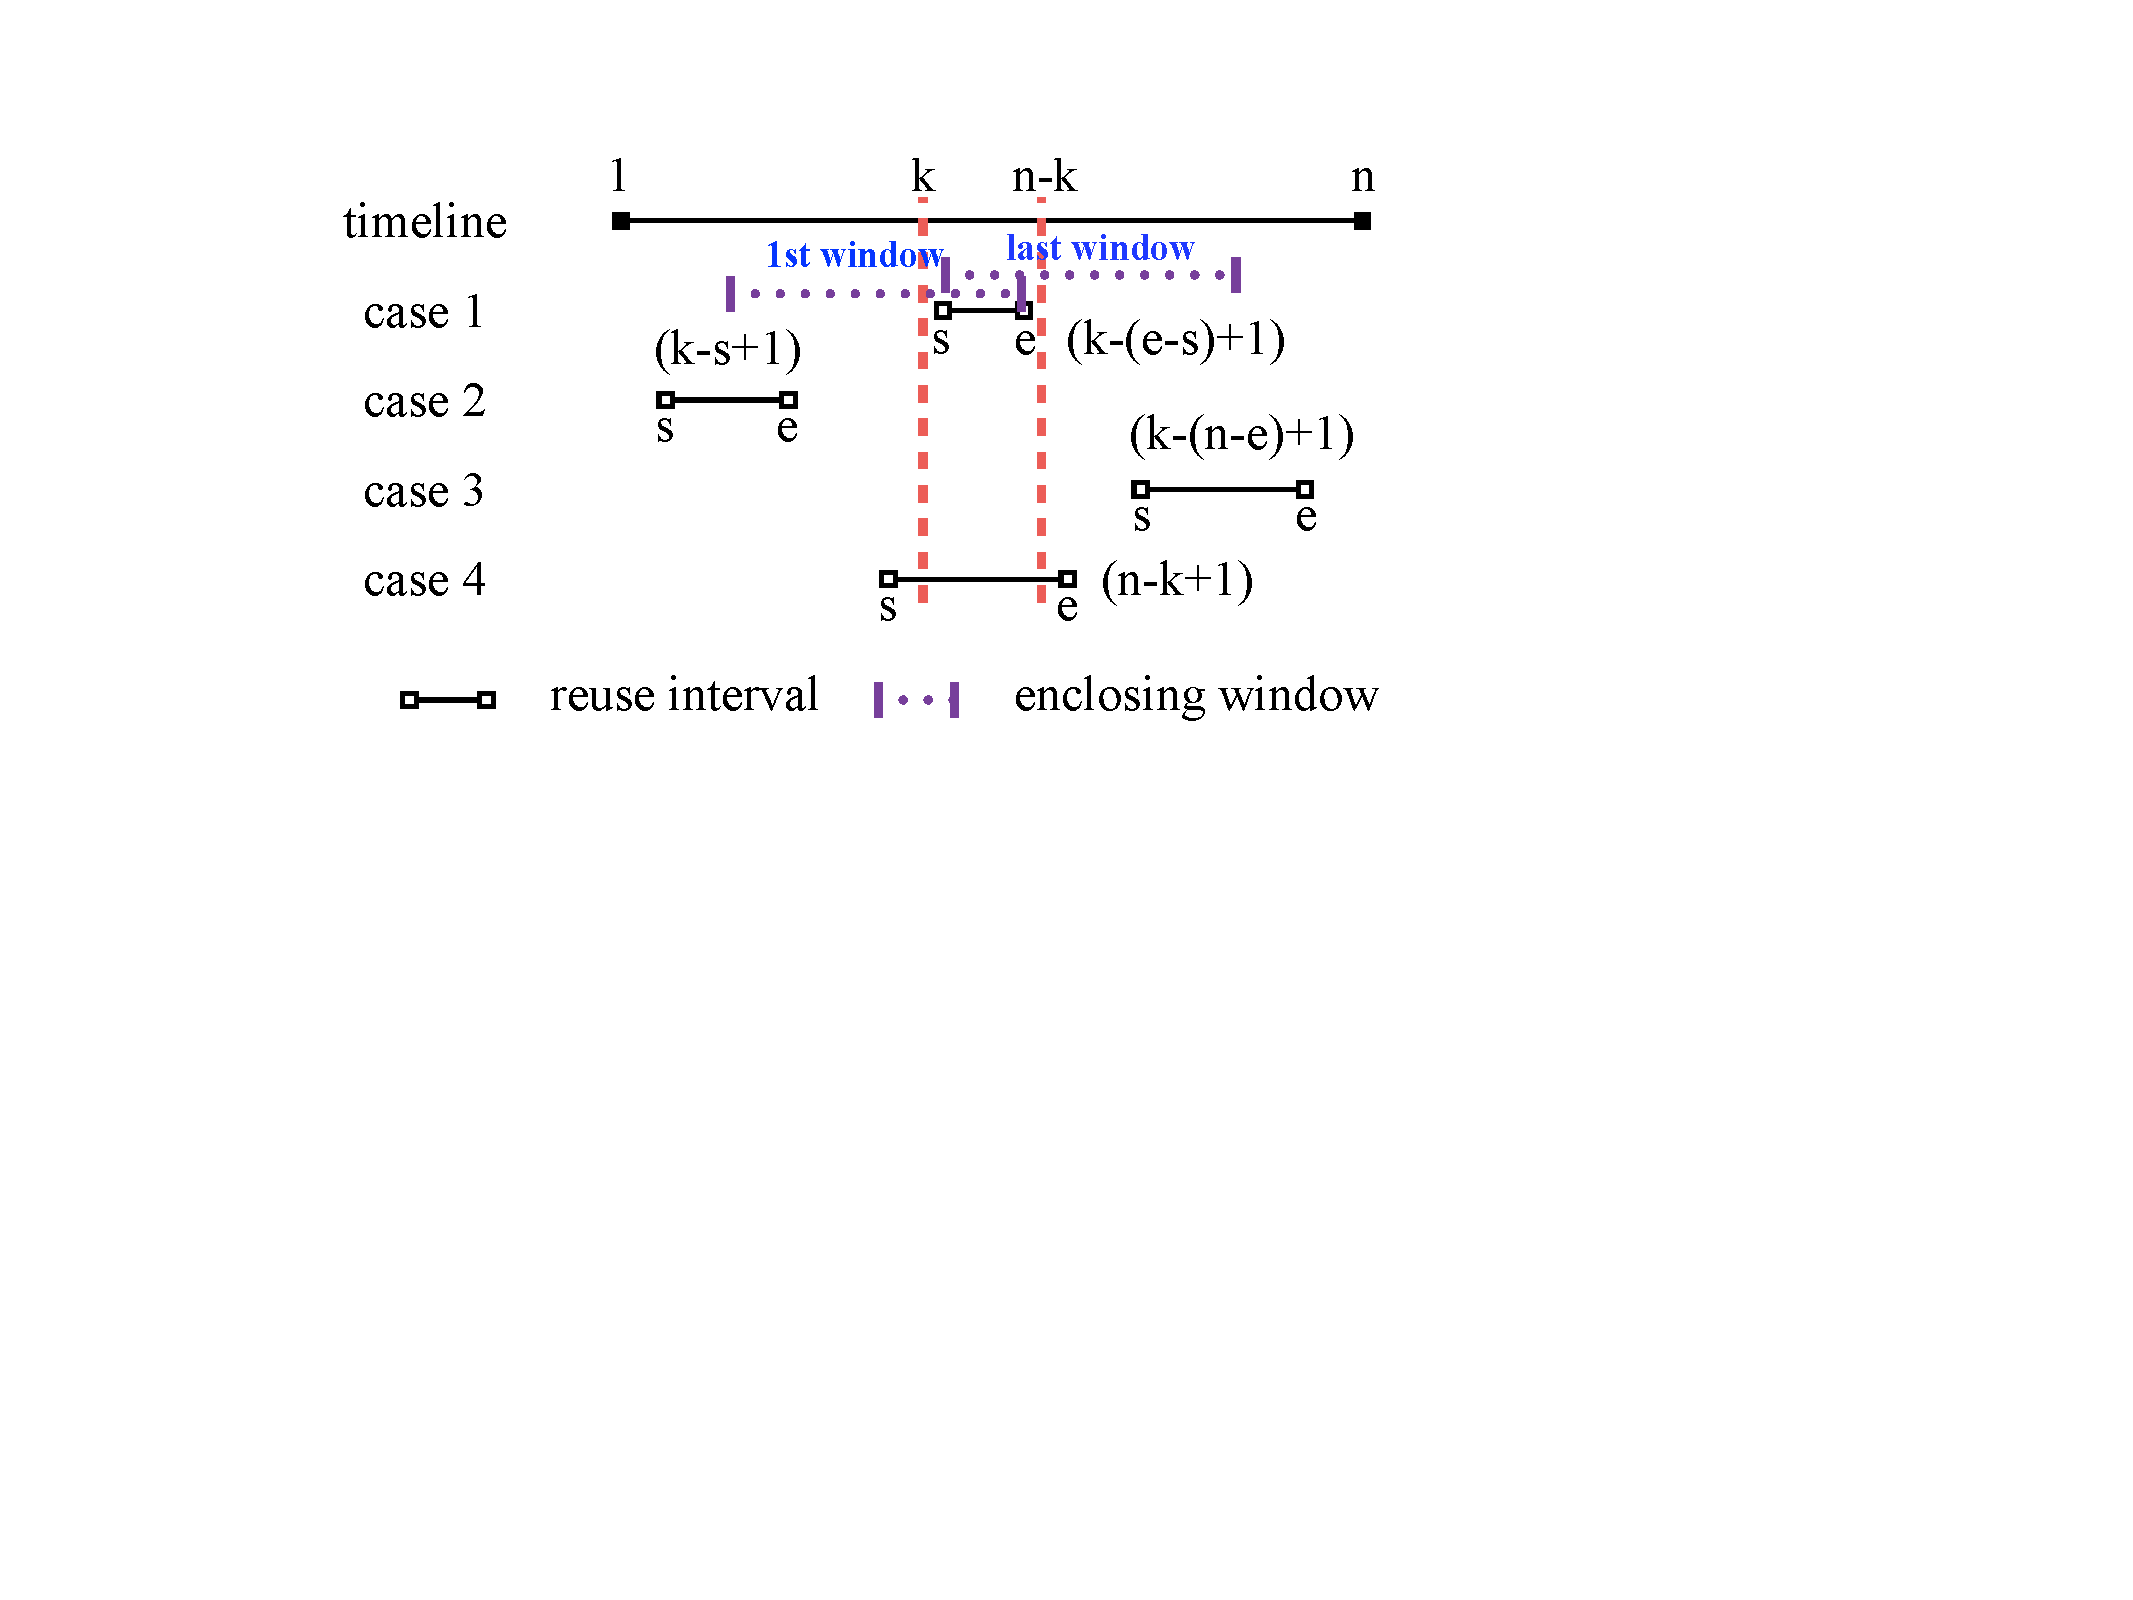
\includegraphics[width=0.4\textwidth]{./figures/reuse_types.pdf}
   \caption{Four cases of counting enclosing windows of a reuse interval.
   The number of $k$-length enclosing windows are written in the parathesis.
   We show the first window and the last window containing the reuse
   interval of case 1.}
   \label{fig:reuse-count}
\end{figure}

Given a trace of length of $n$ and $m$ distinct reuse intervals, $[s_i, e_i]$ 
($i=1 \dots m$), Eq.~\ref{eq:reuse} shows the complete and formal solution. 
The function $I$ is a predicate, which equals to 1 if the condition is true and 
otherwise 0.  In the equation, $I(e_i-s_i\le k)$ counts only reuse intervals not 
longer than $k$.

\begin{equation}
\small
\begin{split}
\textit{reuse}(k) & = \frac{{\sum_{i\textit{=}1}^{m}I(\textit{e}_i\textit{-}s_\textit{i} \le k)(\textit{min}(n\textit{-}k, s_{i} ) \textit{-max} ( k, e_{i} )\textit{+}k\textit{+}1)}}{n-k+1}
\end{split}
\label{eq:reuse}
\end{equation}

The equation reduces time cost from exponential time to quadratic time, since
it takes $O(m)$ time to calculate for each $k$ and $O(mn)$ for all $k$s. 
To further make it linear time, we refer to the algorithm of calculation of all-window 
liveness~\cite{Li+:ISMM14, LiD:MSPC13, DingL:MSPC14}. The liveness
is an existing all-window statistics metric. It counts average number of live objects 
of a window length. Li et al. gave a linear-time algorithm to calculate it. Since
Eq.~\ref{eq:reuse} is quite similar with the liveness formula, we mimic their algorithm.
Due to much similarity, we omit it here.

\subsubsection{Reuse to cache hit ratio}

\emph{reuse(k)} points out the number of reuses of $k$ data accesses, thus there
are \emph{k-reuse(k)} distinct data. Now consider next access after $k$ data accesses. 
The next datum can be either one of the $k$-\emph{reuse(k)} distinct data, or a completely 
different new datum. Literally, \emph{reuse(k+1)} - \emph{reuse(k)} reflects how 
much possibility the next datum falls in the prior \emph{k-reuse(k)} distinct data. Hence, 
\emph{reuse}$'(k)$ represents hit ratio of cache of size ($k$ - \emph{reuse(k)}), as shown in 
Eq.~\ref{eq:reuse2}.
\begin{equation}
\textit{hr(k-reuse(k))} = \textit{reuse(k+1)} - \textit{reuse(k)} = \textit{reuse}'(k)
\label{eq:reuse2}
\end{equation}
\noindent
To understand the relation between reuse and hit ratio, we consider an example
trace ``$abab...$", which is infinitely repeating. The following table shows discrete
values of \emph{reuse(k)} and hit ratio, where $c$ denotes cache size, i.e.  \emph{k-reuse(k)}.
\begin{center}
\begin{tabular}{cc|cc}
$k$ & $reuse(k)$ & $c$ & $hr$ \\ \hline
1 & 0 & 1 & 0    \\
2 & 0 & 2 & 1    \\
3 & 1 & 2 & 1    \\
4 & 2 & 2 & 1   
\end{tabular}
\end{center}
\subsubsection{The correctness of the conversion}

The formal proof of the conversion from reuse to cache hit ratio can be illustrated by 
a recent cache locality theory, called HOTL~\cite{Xiang+:ASPLOS13}. HOTL proves
a higher order relation exists between \emph{footprint}, which counts average number of 
distinct data of a window length, and cache miss ratio, that is, the differentiation of footprint
is cache miss ratio.

\emph{k-reuse(k)} is actually equivalent to footprint according to the definition of footprint.
Thus we have, 
\begin{equation}
\textit{reuse(k)} + \textit{footprint(k)} = \textit{k}
\label{eq:complement}
\end{equation}
\noindent
If we differentiate both sides of Eq.~\ref{eq:complement}, we have 
\begin{equation}
\begin{multlined}
\textit{reuse}'\textit{(k)} = 1 - \textit{footprint}'\textit{(k)} = 1 - \textit{mr(c)} = \textit{hr(c)} \\
\textit{where c is k - reuse(k).}
\end{multlined}
\label{eq:proof}
\end{equation}
\noindent
Eq.~\ref{eq:proof} confirms that our conversion from reuse to cache hit ratio is correct.
HOTL gives a linear-time algorithm to calculate footprint and derive cache miss ratio, 
however it doesn't unveil the relations between reuse and footprint and between reuse 
and cache hit ratio. This work complements the HOTL theory by pointing out that reuse
and footprint are dual metrics of cache locality. This work also provides another linear-time 
algorithm to calculate MRC from the angle of reuse. 

\subsubsection{Dive into the \texttt{Atlas}}

\texttt{Atlas} partitions a program into many FASEs and at the end of FASEs 
the buffered cache lines are flushed out to maintain consistent persistency. 
This semantic requires the adaption of our trace model. 

For example, consider a trace with the consideration of \texttt{Atlas} sematic 
$ab|ab|ab...$, whereby a $|$ denotes an end of a FASE. If we ignore the FASEs, 
the trace fed into our model is $ababab...$. For this trace, \emph{reuse(2)} = 0 
and \emph{reuse(3)} = 1, thus hit ratio of cache of size 2 is 1. However, 
in real, since \texttt{Atlas} flushes out $a$ and $b$ at every $|$, therefore every
access is a miss, whatever cache size actually is. The ignorance of \texttt{Atlas}
semantic results in greater modeled cache hit ratio than real.

To adapt our model to \texttt{Atlas}, we consider the same cache lines in different
FASEs as completely different. In other words, the data in a FASE can not be the same with any 
data in the other FASEs. For example, the above trace will be translated into 
$abcdef...$ and fed into our model.

\subsection{Replacement Policy}
In principle, the software cache is independent of any cache replacement policy. 
However we choose LRU for the time being. On the one hand, LRU is one of the 
most effective replacement policies for cache design, no matter in hardware 
or in software, such as the Memcached~\cite{Fitzpatrick:2004} web cache. On the other hand,
the higher order relation between reuse and cache hit ratio holds only
for LRU replacement policy, which was proved by HOTL~\cite{Xiang+:ASPLOS13}.
In the future, we will study other replacement policies. So long as they have
effective means to construct MRC, we can enrich the software cache.

\subsection{The Expiration List}
\label{sec:exp}
Large cache size, while decreasing cache miss ratio, hurts performance, since
flushing many cache lines at a time at the end of FASEs stalls CPU computation. 
To alleviate the performance issue caused by large cache size, we design a sorted 
list, called \emph{the expiration list},  to evict cache lines in advance.

We assign an expiration time to a cache line when put into the software cache.
The expiration time is ``access time + \emph{cache fill time}~\cite{Xiang+:ASPLOS13}".
The cache fill time of cache size $c$ is the time window length $k$ such that 
\emph{k-reuse(k)} = $c$, that is, the window length when footprint equals to $c$. 
It implies how long a datum stays in the cache on average. Thus the rational
is that if a cache line stays longer than cache fill time, it is highly possible that
the cache line is not used any more. The expiration time is frequently updated
every time upon a memory store. The cache fill time is variable at runtime. 

We periodically check the expired. If cache size is small, it costs little to flush the 
whole software cache at a time, thus it matters little that whether we can flush a 
couple of unused cache lines ahead of time. Therefore, the period to check can be set 
long. On the contrary, the period is set to be short, if cache size is large, since 
the cost of flushing the whole software cache is huge and frequent checking is 
necessary.

The expiration list has two advantages. One is to utilize rich memory bandwidth 
at appropriate times to overlap computation and memory transfer. The other is 
that fewer cache lines than the software cache size are flushed out at the end 
of FASEs.

\subsection{System Implementation}
% TODO 
% not clear. Many places are not clear.
% when to update cache fill time.

\paragraph{The software cache} 
The software cache is thread-specific. We dedicate the implementation to $O(1)$ time.
We adopt the data structure of a hash map plus a double-linked list. The
double-linked list actually implements the software cache. Each node 
denotes a cache line. The hash table maps the address of a cache line 
to the corresponding node in the double-linked list. The frequent operations 
for a cache are LRU-based updates. The hash map is used to search a cache 
line in $O(1)$ time, without having to traverse the list in $O(n)$ time. With 
the data structure, insertion, update and deletion for cache lines are all $O(1)$ 
time. The data structure borrows the idea of the data structure used in Linux 
OS in managing pages, where a red-black tree for insertion, update and deletion 
of pages and a double-linked list for traversal are used. We are even faster 
by using a hash map rather than a red-black tree. Figure~\ref{fig:system}
shows the data structure of the software cache.

\begin{figure}[hbpt]
\centering
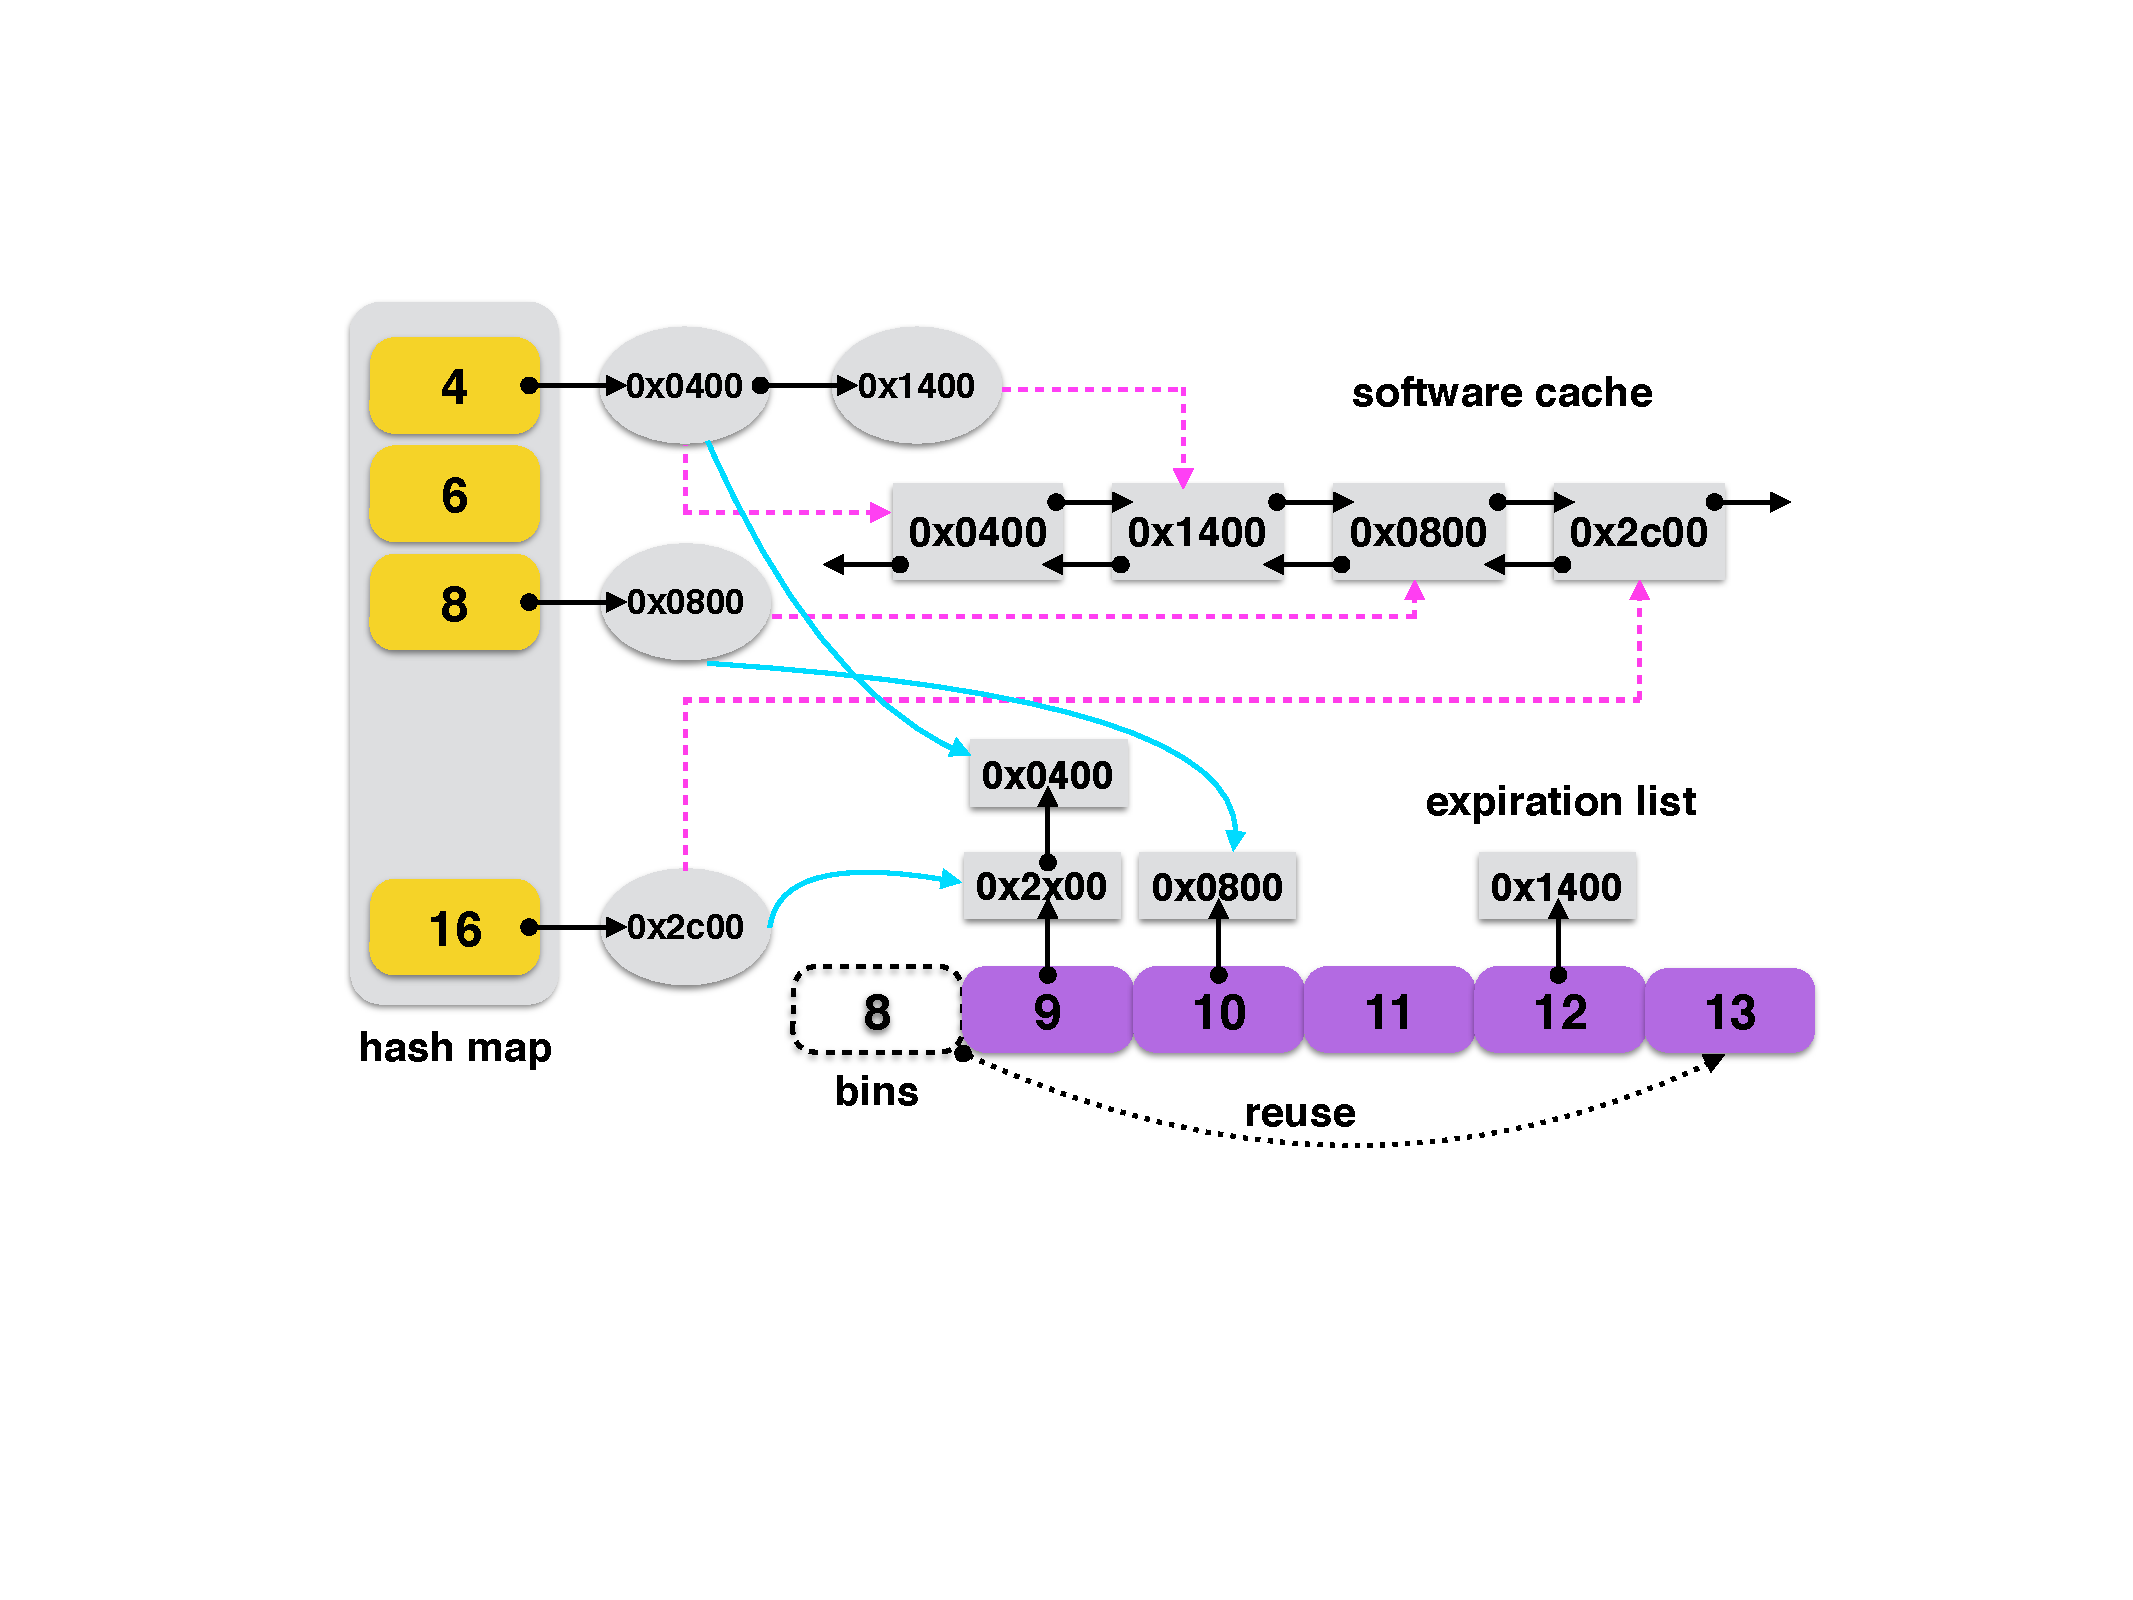
\includegraphics[width=8.5cm]{figures/system.pdf}
\caption{The system design of the software cache. The red dashed line denotes 
mapping from the address of a cache line to a node in the software cache. The blue
solid line denotes mapping from the address of a cache line to a node in the expiration
list. The numbers in the hash map are hash keys. The numbers in the array of bins are
expiration times. All the remaining numbers are all cache line addresses.}
\label{fig:system}
\end{figure}

We maintain an array of bins to implement the expiration list. Each bin 
contains a singly-linked list of cache lines with the same expiration time. 
Each bin is indexed by the expiration time. All bins are sorted in the 
ascending order of expiration time. Figure~\ref{fig:system} shows the data 
structure organization. We periodically check whether the first bin expires. 
If it doesn't expire, we do nothing. Otherwise, we start to flush the bins 
along the array until we meet one bin that doesn't expire. The flushed 
bins can be reused in the future for the cache lines with new expiration time. 
Therefore the array of bins is actually a circular buffer. This design dispels
the doubt that infinite expiration time may cause infinite length of the array
of bins, which is not doable. The rational behind this is that array 
length is bounded by cache fill time, thus not infinite. We call it a locality-inspired 
design. 

During program execution, an access to the software cache requires 
to update its expiration time.  To search an existing cache line in the expiration
list in $O(1)$ time, we reuse the hash map designed for the software cache. 
The hash table also maps a cache line to a node in the expiration list, as 
shown in Figure~\ref{fig:system}. Hence, insertion, update and deletion of the 
expiration list are all $O(1)$ time.

The design has another merit. For any insertion of a cache line or update of 
the expiration time of an existing cache line, it costs $O(1)$ time. We only
need to link the cache line to the corresponding bin. This is significantly 
important, since the expiration time of a cache line is frequently updated. 
If we use a sorted singly-linked list to organize the cache lines and their 
expiration times, which is a much simpler design, it costs $O(n)$ time to 
traverse the list to find the right position to insert a cache line in, where 
$n$ is the list length. In fact, the sorted array of bins implies a totally 
sorted linked list of all cache lines. 

\paragraph{Offline and online MRC analysis}
One way to utilize MRC is offline selection of cache capacity, and then the software
cache is a profiling-based approach. The chosen cache capacity is generally 
the best from the whole-program point of view. The offline calculation is linear time. 

Online MRC analysis requires $O(1)$ time efficiency. We borrow the bursty sampling 
approach~\cite{ArnoldR:PLDI01,ChilimbiH:PLDI02} to implement it. The approach partitions 
program execution into burst periods and hibernation periods.  At burst periods, we record the 
meta-data, for example reuse intervals, used to compute MRC, which costs $O(1)$ time. 
At the end of a burst period, we calculate MRC, and then adjust the cache capacity 
and cache fill time, accordingly. Though the calculation of MRC is linear time, the amortized 
time is $O(1)$. Nothing needs to be done at hibernation periods. The time complexity of the 
worst-case, when the hibernation period is 0 long, is $O(1)$. In practical, we specify long 
hibernation period to further reduce time cost. This works well when a program has few 
phase changes. For instance, we specify infinite long hibernation period for our tested 
programs, which means we only run MRC calculation once. Results show that the cache 
sizes selected by sampling MRC is sufficiently good and the overhead of MRC calculation 
is very low. 

\paragraph{Compiler support} 
We implemented a pass in LLVM~\cite{LattnerA:PLDI05} to instrument all memory 
stores, locking, and unlocking operations. The instrumented memory stores are fed
into the software cache. The locking and unlocking operations are instrumented to
label FASEs.

\section{Evaluation}

\subsection{Methodology and Platform}

\paragraph{Methodology}

Intel recently announced that its non-volatile memory technology 3D XPoint~\cite{3DXPoint:2014} will 
be put into product next year. Because real non-volatile memory is not yet available, 
DRAM was used to simulate non-volatile memory. Linux \texttt{tmpfs} [32] was used 
for ``persisting" data. The data on \texttt{tmpfs} is directly memory-mapped into the 
address space when a process launches and can be completely backed up by DRAM 
when a process terminates. Hence, \texttt{tmpfs} provides a directly mapped, 
byte-addressable persistent memory across process terminations, which exactly 
mimics the functionality of non-volatile memory for persistence across machine crashes.

Based on this experimental setup, we compare the software cache approach with
other approaches that provide consistent data durability. We will also compare with
the approach which doesn't provide data durability to demonstrate the tradeoff between
performance and persistence.

We compare with four approaches. The first approach is the state-of-the-art work,
the \texttt{Atlas} approach~\cite{Dhruva+:OOPSLA14} ({\bf AT}), as stated in Section~\ref{sec:back}. 
The second approach is the optimal approach ({\bf BEST}), which achieves the maximal 
overlap of cache line flushes and the optimal flush scheduling to overlap computation 
and memory transfer maximally, i.e. the best performance with the guarantee of consistent
data durability. Since we are not aware of the optimal solution, we use the approach,
which doesn't flush any cache lines, to represent it. Obviously, it is the upper bound of 
the optimal solution. The third approach is the eager ({\bf ER}) approach, which flushes 
cache lines instantly every time a persistent store happens. The fourth approach is the 
lazy ({\bf LA}) approach, which flushes all cache lines until the end of transactions.

For reproducible results, we use a second-run method, which is to first 
profile MRC offline and then after selecting the best cache capacity, 
test the performance in the second run, for all programs. Online analysis 
will be fast because we have $O(1)$ design. To confirm so, we show 
the runtime overhead of sampling MRC in Section~\ref{sec:ove}.
This measurement adoption has another merit, which additionally tells 
the performance breakdown of the software cache system. We select 
the smallest cache size which has less than 1\% cache miss ratio.
Results are all averages over 3 runs. 

\paragraph{Platform}
We performed all experiments on a machine shipped with 60 Intel Xeon E7-4890 cores at 2.8GHz, 
running Linux OS 3.10. 

\subsection{Applications}

\paragraph{Micro-benchmarks}
To understand the cost of cache line flushes and importance of selection of cache size, 
we start with a simple sequential program \emph{persistent-array}. It has only one durable
transaction, which consists of a two-level nested loop. The inner loop iterates 400 times and
writes, in the iteration $i$, to the $i$-th element of an array of integers. The outer loop 
repeats the inner loop 2500 times. On the tested machine, a cache line, size of 64 bytes,
holds 16 4-byte integers. Therefore, the inner loop accesses 25 (cache line aligned) or 26 
(not cache line aligned) cache lines. \texttt{Atlas} uses table size of 8. Due to cache spatial 
locality, around $15/16$ data flushes are optimized away by \texttt{Atlas}. Hence, its data 
flush ratio is 0.0625, as shown in Table~\ref{tbl:bench}. However, the software cache approach 
captures the best cache size, 26, which further optimizes the data flush ratio to only 0.00003, 
that is the flushed 26 cache lines in total. Figure~\ref{fig:model-appendix} shows that cache
size of 26 has a cache miss ratio of 0.00003, i.e. the data flush ratio of 0.00003.

The \emph{queue} is a multithreaded benchmark we wrote based on the blocking algorithm
of Michael and Scott~\cite{MichaelS:PODC96}. The \emph{hash} is a single-threaded
open-source hash table~\cite{Clark:2005}. The singly \emph{linked-list} is a multithreaded
benchmark, whereby a total of $N$ elements are inserted in a perfect shuffle pattern
with a configurable number of elements added atomically at each step. These data
structures are often used for dynamic irregular programs. We measured them to show 
the challenge of maintaining persistence for these types of programs while wanting
good performance. 

\paragraph{SPLASH2 benchmark suite}
All applications, but \emph{radiosity}, from SPLASH2~\cite{Woo+:ISCA95} benchmark
are evaluated. We have a compile error on \emph{radiosity}. The basic statistics of
SPLASH2 benchmark is shown in Table~\ref{tbl:bench}. Variations shown by problem
sizes and the number of FASEs demonstrate that they are good representative. 
We persist all data structures in SPLASH2 that are not stack-allocated to create
the worst-case for data durability, since the cost of durability is often proportional 
to the amount of persisted data~\cite{Dhruva+:OOPSLA14}, and then to give us a fair 
idea of the performance we are able to obtain while maintaining the worst-case 
consistent durability.

\paragraph{Memory-mapped database (MDB)}
MDB~\cite{Chu:2014} is an in-disk key-value store based on B-tree to service
the OpenLDAP~\cite{OpenLDAP} backend. MDB supports transactions and uses MultiVersion
Concurrency Control (MVCC). A memory-mapped file of in-disk key-value pairs 
is used for gets and puts. Readers start with the snapshot at the beginning of a 
transaction and run in parallel with writers. Writers use copy-on-write policy. 
A reader always sees a valid B-tree without having to acquire locks. While,
a write transaction requires to acquire a lock to exclusively from other writers
to update an old version to a new version. Therefore, read transactions
don't imply many FASEs, while write transactions do. MDB gives us a sense 
of tradeoff between persistence and performance in the cloud-level applications.

\subsection{The Data Flush Reduction}
\begin{table*}
\small
\centering
\begin{tabular}{|c|c|c|c||c|c|c|c|c|c|}
\hline
{\bf Benchmarks} & {\bf Problem Size} & {\bf Total FASEs}& {\bf Total Flushes} & {\bf ER} & {\bf LA} & {\bf AT} & {\bf SC} & {\bf AT/SC} & {\bf SC/LA} \\ \hline \hline
linked-list & 10000 & 10K & 49999 & 1.00000 & 0.60001 & 0.60001 &  0.60001 & 1$\times$ & 1$\times$ \\ \hline
persistent-array & 100000 &  1 & 1000001 & 1.00000 &  0.00003 & 0.06250 & 0.00003 & 2083.333$\times$  & 1$\times$  \\ \hline
queue & 400000  & 0.3M &  400006 & 1.00000 &  0.62500 & 0.62500 & 0.62500 & 1$\times$  &  1$\times$  \\ \hline
hash & 4000 & 7K & 83061 & 1.00000 & 0.50092 & 0.62128 & 0.59531 & 1.044$\times$  & 1.188$\times$  \\ \hline
barnes & 16384 & 69K & 270762562 & 1.00000 & 0.00295  & 0.08206 & 0.00391 & 20.987$\times$  & 1.325$\times$  \\ \hline
fmm & 16384 & 43K & 87711754 & 1.00000 &   0.00246 & 0.01683 & 0.00328 & 5.131$\times$  & 1.333$\times$  \\ \hline
ocean & 1026 & 648 & 25242763 & 1.00000 & 0.09203  &  0.40290 & 0.16467 & 2.447$\times$  &  1.789$\times$  \\ \hline
raytrace & car & 346K & 65509589 & 1.00000 &  0.07140 &  0.13952 & 0.07918 & 1.762$\times$  & 1.108$\times$  \\ \hline
volrend & head & 45  & 391692398 & 1.00000 & 0.00219 &  0.03189 & 0.00219 & 14.561$\times$  & 1$\times$  \\ \hline
water-nsquared & 512 & 2.1K & 45338822 & 1.00000 & 0.00107 & 0.05334 & 0.00411 & 12.978$\times$  & 3.748$\times$  \\ \hline
water-spatial & 512 & 77 & 40981496 & 1.00000 & 0.00103 &  0.07122 & 0.00157 & 45.363$\times$  & 1.524$\times$  \\ \hline
mdb & 3000 & 3.6K & 274609 & 1.00000 & 0.50832 & 0.66966 & 0.57760 &1.159$\times$  & 1.136$\times$  \\ \hline \hline
average & - & 65.1K & 77420588 & 1.00000 & 0.20061 & 0.28135  & 0.22071 &  182.565$\times$ & 1.427$\times$ \\ \hline

\end{tabular}
\caption{The benchmark statistics and results of data flush ratios of different approaches.}
\label{tbl:bench}
\end{table*}

Table~\ref{tbl:bench} shows statistics of all tested programs under certain problem sizes.
The number of FASEs ranges from 77 to 0.3M and the number of cache line flushes 
ranges from 50K to 391M, showing that they can represent a wide range of program 
characteristics. 

Since ER immediately flushes a cache line when a persistent memory store 
finishes, the data flush ratio of ER is 1.0. LA  overlaps all cache line flushes that
can be overlapped within a FASE, thus the data flush ratio reaches the minimum.
LA suggests that even if a program has tons of data persisted, for example the \emph{volrend}
with 391692398 flushes, it is possible to extremely largely reduce them.
However, since all cache line transfers to memory are performed at the end of 
FASEs, CPU resources are wasted and thus performance is extremely bad. As tested,
for some programs, LA performance can be hundreds of times worse than \texttt{Atlas}.
Hence, in this evaluation, we only show the data flush reduction of LA  to
give a lower bound for comparison. 

AT and SC are in the middle of ER and LA. AT hugely reduces data flushes by
using a fixed table size of 8, but there is still big room to improve. On average,
SC further reduces data flushes by $183\times$. Even excluding the micro-benchmark
\emph{persistent-array}, SC outperforms AT by around $10\times$ significantly for 
the remaining programs. The result confirms the significance of selection of the best 
cache size. In Section~\ref{sec:mrc-res}, we will give
the chosen cache sizes are all different. Unfortunately, SC is not better than AT on 
\emph{linked-list} and \emph{queue}. The essence is that AT and SC both reduce to 
minimum on the two programs, which can be known by comparing with LA.

The comparison with LA lets us know how good SC is. SC is only a little worse than LA,
roughly by $42\%$ on average. The result greatly demonstrates that SC is very effective
in the performance optimization for data persistence. On \emph{volrend}, which has
the most data flushes, SC even reaches the optimal.

\subsection{The MRC Prediction Precision}
\label{sec:mrc-res}

\begin{figure}[hbpt]
\centering
\subfloat {
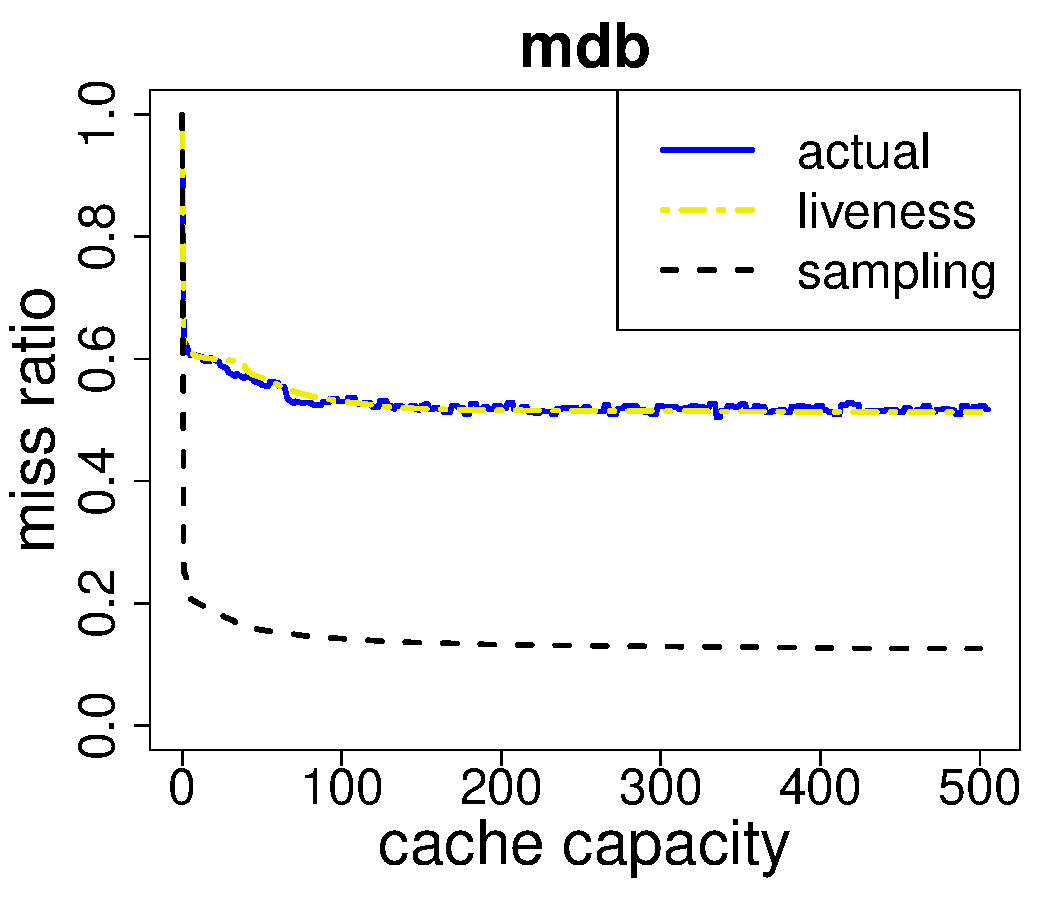
\includegraphics[width=4.3cm]{./figures/mdb_new.pdf}
\label{fig:simplutoco}
}
\hspace*{-1em}
\subfloat {
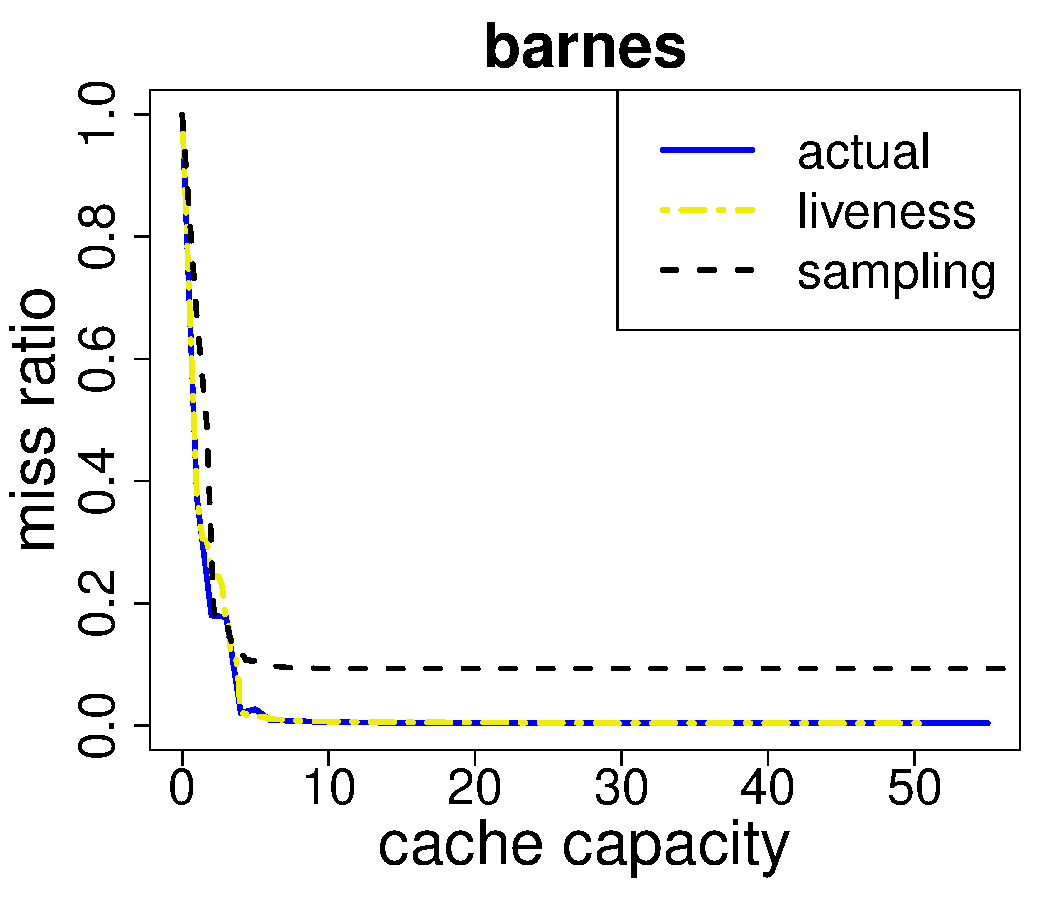
\includegraphics[width=4.3cm]{./figures/barnes_new.pdf}
\label{fig:simplutosolo}
}
\vspace*{-1em}
\\
\subfloat {
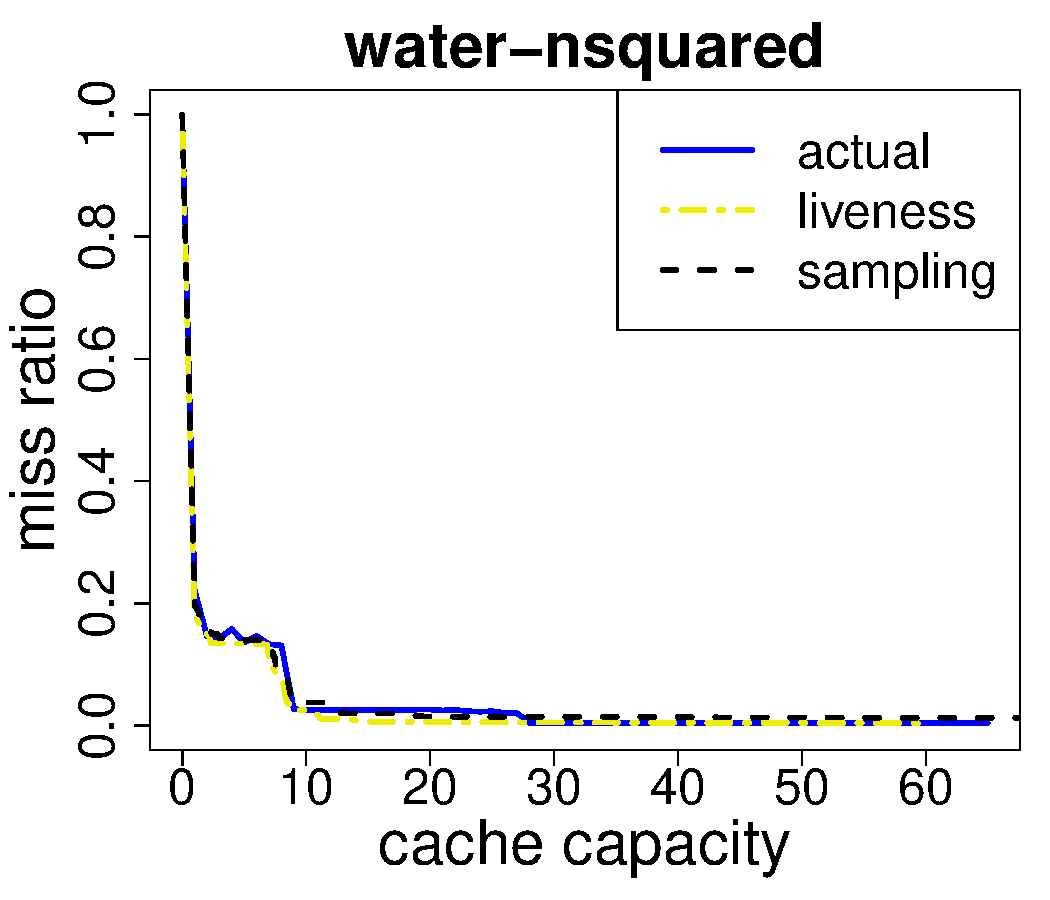
\includegraphics[width=4.3cm]{./figures/water-ns_new.pdf}
\label{fig:simplutoco}
}
\hspace*{-1em}
\subfloat {
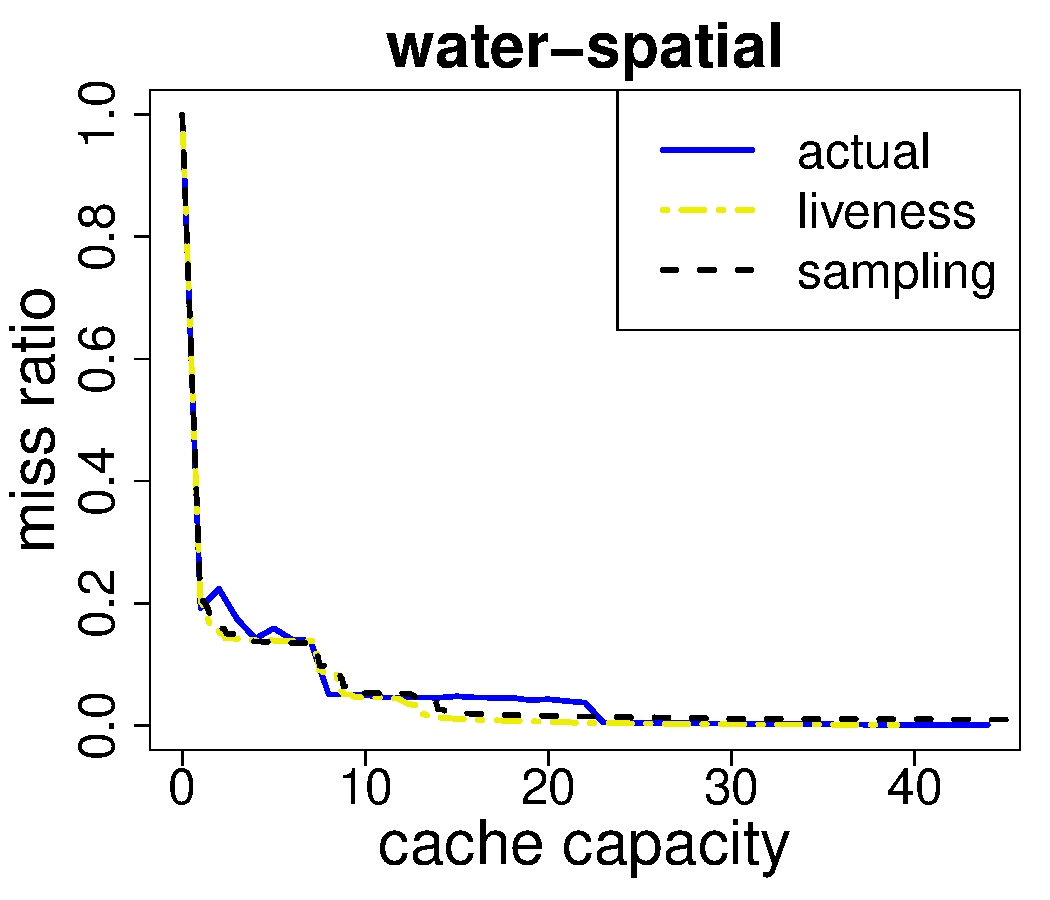
\includegraphics[width=4.3cm]{./figures/water-sp_new.pdf}
\label{fig:simplutosolo}
}
\caption{The comparison between actual MRC, accurately modeled
MRC and sampling MRC, of four programs.}
\label{fig:model}
\end{figure}

Figure~\ref{fig:model} shows the effectiveness of our model in predicting MRC by four
programs. The MRCs of the other programs are listed in Figure~\ref{fig:model-appendix}
in Appendix. Results first turn out that our model is quite precise in predicting MRC for all programs but 
\emph{ocean} program. In \emph{ocean}, our predication drops earlier than the actual
MRC. 

Based on MRCs, the selected cache sizes of \emph{barnes}, \emph{fmm}, \emph{ocean}, 
\emph{raytrace}, \emph{volrend}, \emph{water-nsquared}, \emph{water-spatial}
\emph{mdb} are 15, 10, 2, 8, 3, 28, 23 and 29, respectively. Surprisingly, these small
cache sizes have so small data flush ratios in Table~\ref{tbl:bench}. In addition, we can
see that there is no one-fits-for-all solution for cache size selection. Cache size needs to be
workload-aware. This is a significant reason that SC outperforms AT.

Sampling MRC is not as precise as the accurate MRC. But in terms of cache 
size selection, it is good enough. Because sampling MRC almost has knee points 
at the same x-axis values as accurate MRC. We will show that its overhead is negligible later,
which makes it an online analysis.

\subsection{The Performance}

\begin{figure}[hbpt]
\centering
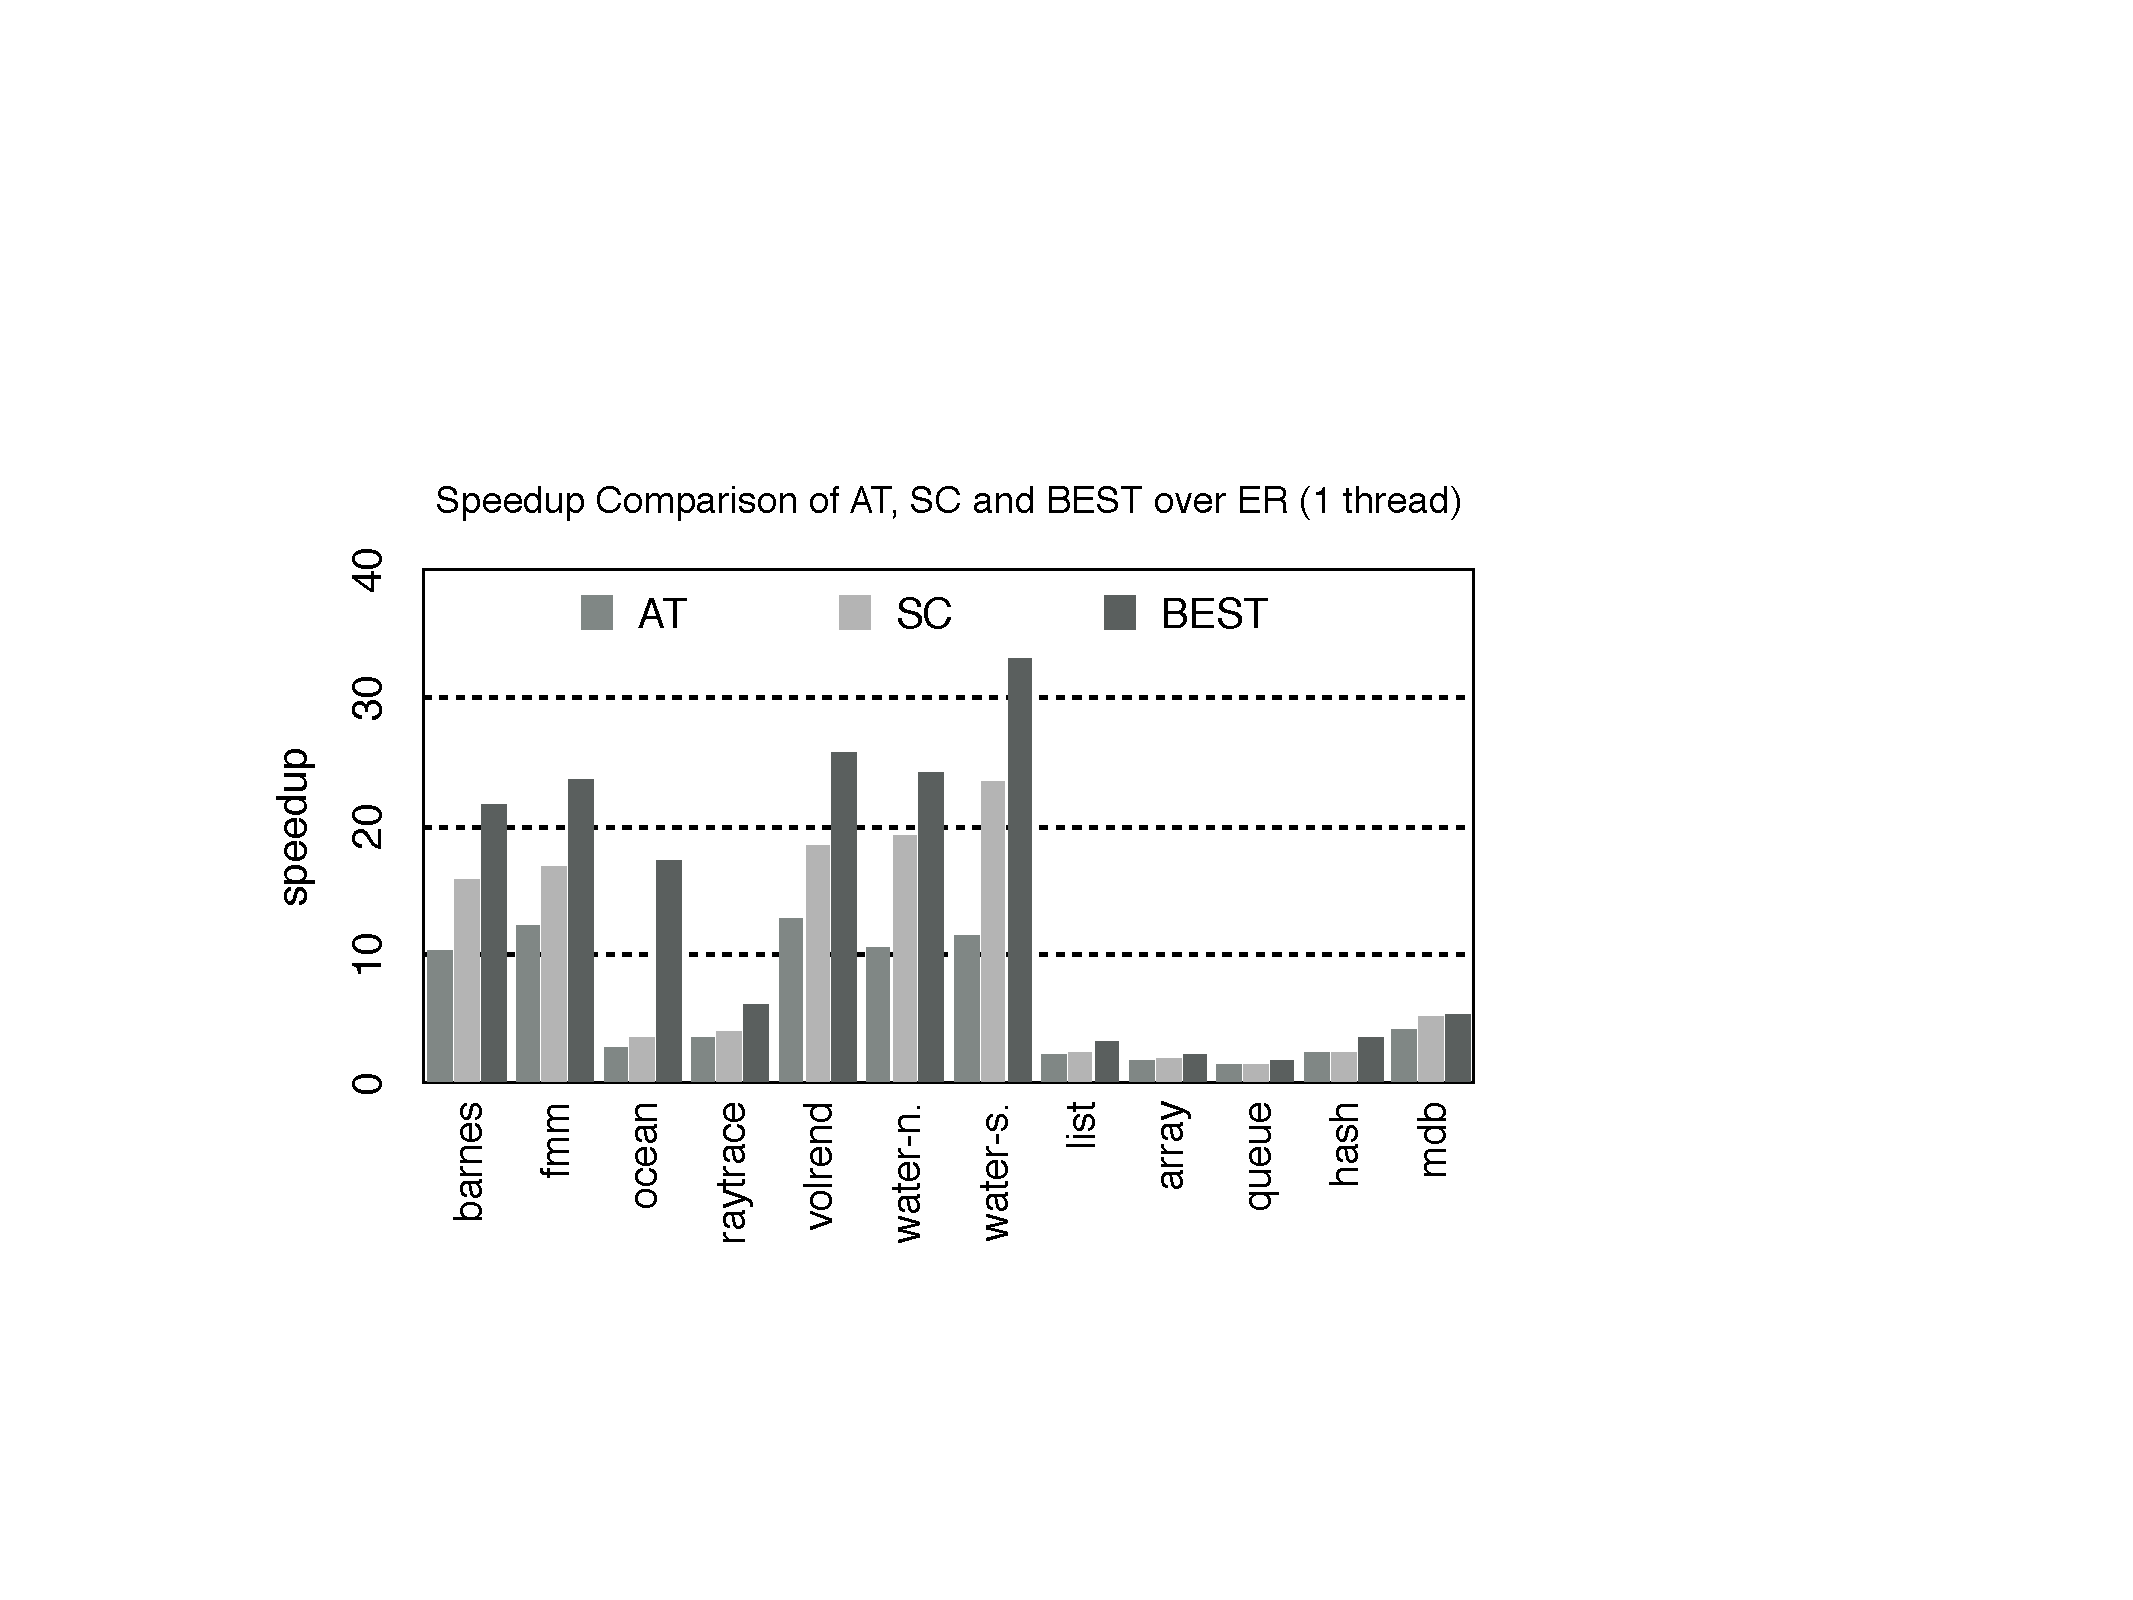
\includegraphics[width=8.5cm]{figures/perf_comp1.pdf}
\caption{Performance comparison between ER, AT, SC and BEST for
1 thread run. We normalize to ER. \emph{water-n.} denotes \emph{water-nsquared}.
 \emph{water-s.} denotes \emph{water-spatial}. }
\label{fig:perf1}
\end{figure}

The performance is measured by execution time. Figure~\ref{fig:perf1} compares
the performance of ER, AT, SC and BEST approaches for 1 thread run. 
Over ER, the speedup of SC ranges from $1.5\times$ to $23.5\times$, with an average of $9.6\times$. 
Over half of them are over $5\times$, 30\% are more than $15\times$, and 
over 10\% are over $19\times$. The greatest speedup, $23.5\times$, is \emph{water-spatial} 
program. AT is also much faster than ER, by $6.3\times$ on average.

SC is uniformly better than AT. The average speedup over AT is $1.4\times$ and the
greatest speedup reaches $2.1\times$ on \emph{water-spatial} program, and the
smallest speedup is $1.01\times$ on \emph{hash}. The data flush ratio reduction
shown in Table~\ref{tbl:bench} explains the reason that SC significantly outperforms 
AT. On \emph{linked-list} and \emph{queue}, although SC has the same data flush ratios
as AT, since smaller cache sizes are used, SC saves time by flushing fewer cache lines at the end of FASEs.

BEST is the fastest, since it doesn't involve any cache line flushes. It is even
faster than the optimal approach, as discussed before. That SC is only $62\%$ worse than 
BEST on average shows that the software cache approach is competitive for performance with
the guarantee of consistent data durability. We believe that if comparing with the optimal 
cache-flushing approach, SC is more optimistic. The \emph{ocean} is the worst, near 
$4.8\times$ slowdown. In \emph{water-nsquared}, SC is very close to BEST, near 81\%.

\begin{figure}[hbpt]
\centering
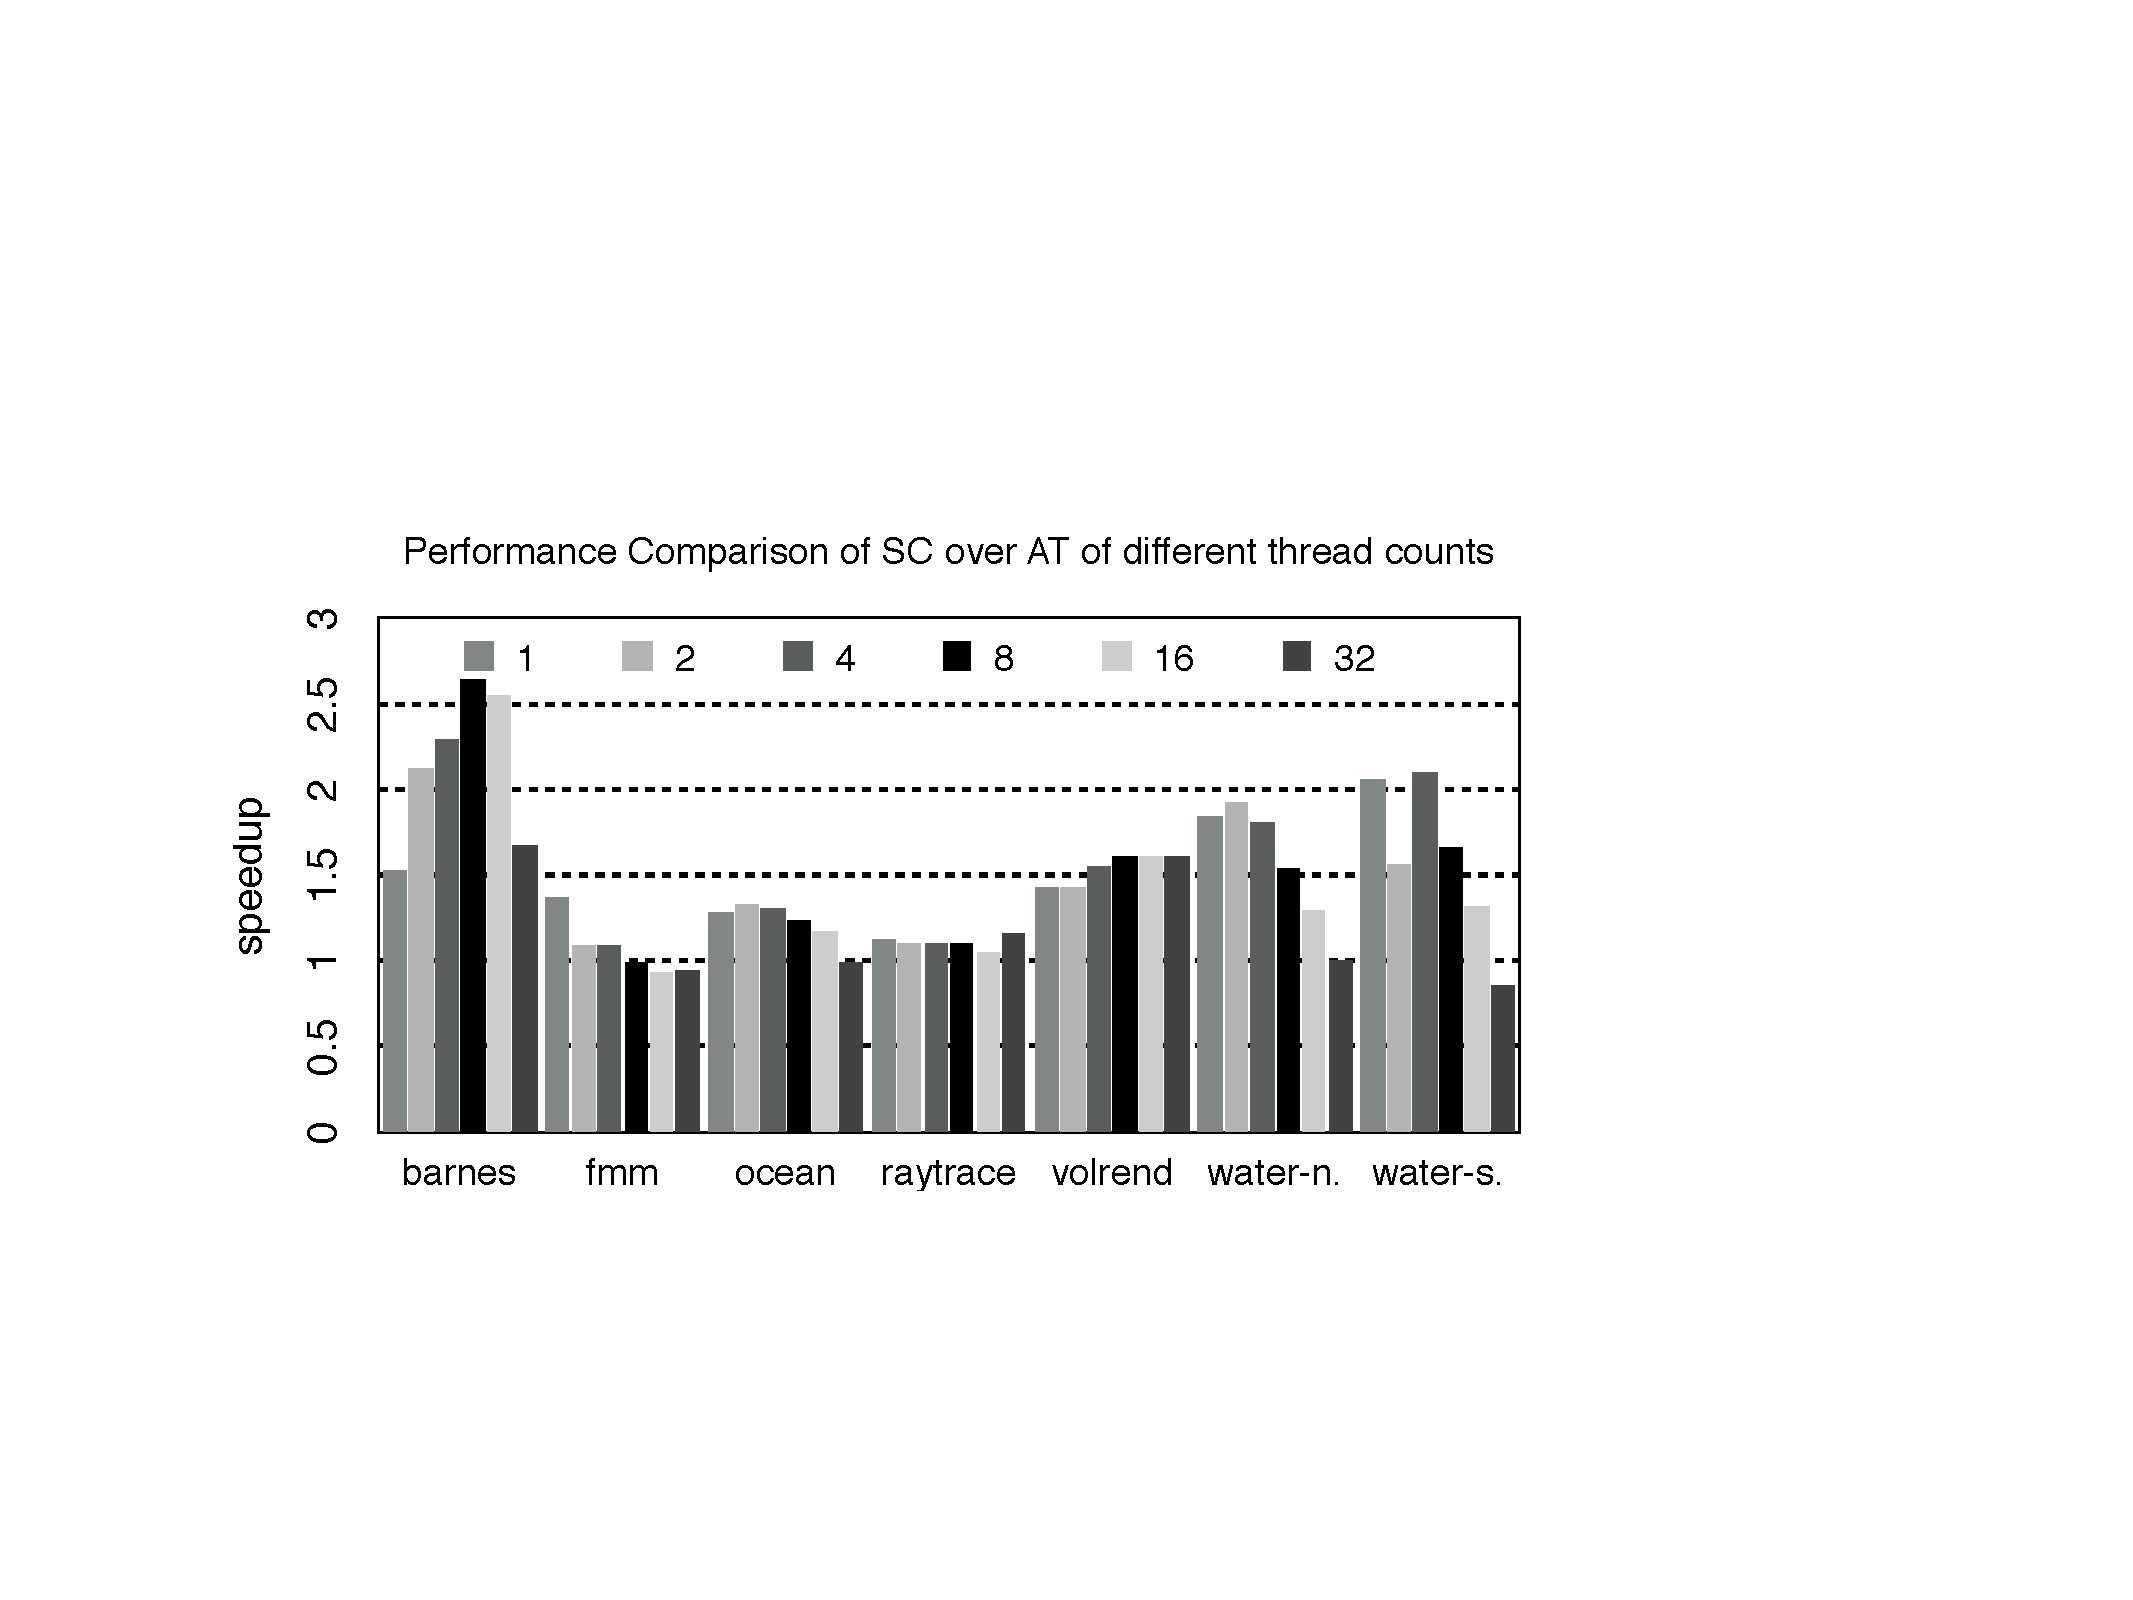
\includegraphics[width=8.5cm]{figures/perf_sc2at.pdf}
\caption{Performance comparison between AT and SC for different numbers 
of threads.  \emph{water-n.} denotes \emph{water-nsquared}.
 \emph{water-s.} denotes \emph{water-spatial}. }
\label{fig:perf2}
\end{figure}

Figure~\ref{fig:perf2} compares SC and AT for different thread counts from 1 to 32.
In 90\% (38 out of 42) of tests, SC is better than AT. The greatest speedup is $2.65\times$ on
\emph{barnes} when thread count is 8. In particular, SC uniformly outperforms AT 
for all programs at small thread counts from 1 to 8. SC is better than AT at large thread counts
for most programs but \emph{fmm} and \emph{ocean} at thread count of 16 and \emph{fmm} 
and \emph{water-spatial} at thread count of 32. One possible reason for these few programs 
to be worse at thread counts of 16 and 32 is that SC worsens the data locality at large thread 
counts as a result of a larger memory footprint than AT due to the software cache is much more 
complicated than \texttt{Atlas}'s approach in implementation. However, it doesn't imply that the 
scalability of SC is poor (discussed in Section~\ref{eval:sca}). Instead, it indirectly shows that 
scalability of AT is very good. The speedups of \emph{barnes}, \emph{raytrace} and 
\emph{volrend} take a general increasing trend when thread count gets larger. 

As the expiration list is primarily designed to prevent CPU from being idle for
large cache sizes, we don't gain performance from the expiration list for current tested programs,
which only need cache sizes of less than 30. Instead, it incurs performance overhead.
However, since the period to check expired is long for small cache sizes, the increased 
overhead is very little, around 2.6\%. Even with this overhead, SC is still better than AT. 
This just illustrates our design is flexible and highly efficient. In the long run, the expiration
list is useful because of its $O(1)$ time efficiency.

\subsection{The Scalability}
\label{eval:sca}

\begin{figure}[hbpt]
\centering
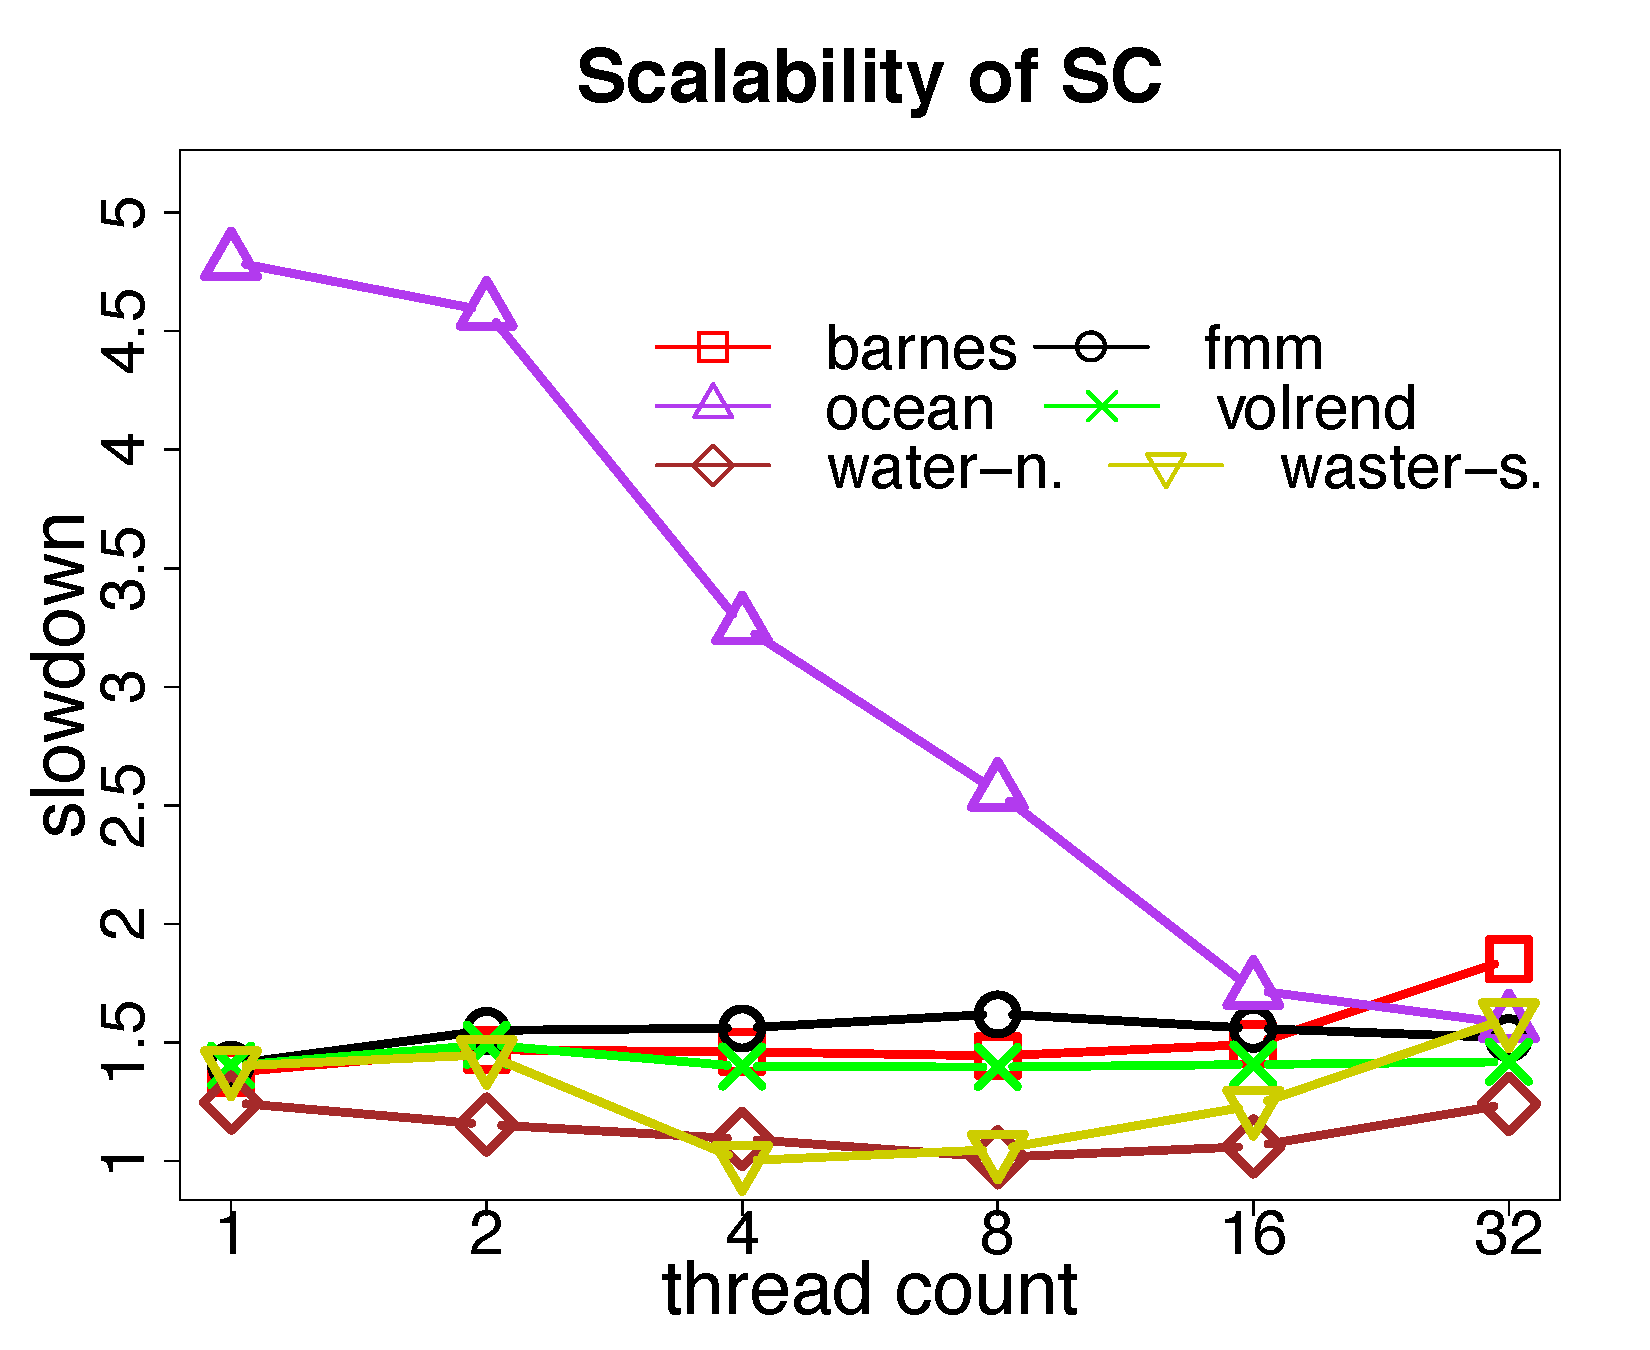
\includegraphics[width=7cm]{figures/scalability.pdf}
\caption{Scalability results of SC. \emph{water-n.} denotes \emph{water-nsquared}.
 \emph{water-s.} denotes \emph{water-spatial}. }
\label{fig:scala}
\end{figure}

The scalability is measured by the performance slowdown of SC over BEST.
This measurement is to avoid the bias of bad scalability of a program itself.
That performance slowdown stays the same or gets decreased means a well
scalability. Figure~\ref{fig:scala} shows scalability results of 6 programs. There
was a running error for \emph{raytrace} for BEST. \emph{Ocean} has a super
linear scalability since its performance slowdown gets decreased and the scalability of the
other programs are all good from thread count of 1 to 16. For \emph{barnes},
and \emph{water-nsquared}, performance slowdown gets subtly increased at thread count
of 32. The phenomenon is consistent with that the speedup of SC over AT is smaller at
large thread counts for the two programs due to large memory footprint.


\subsection{The Overhead of Sampling MRC}
\label{sec:ove}

\begin{figure}[hbpt]
\centering
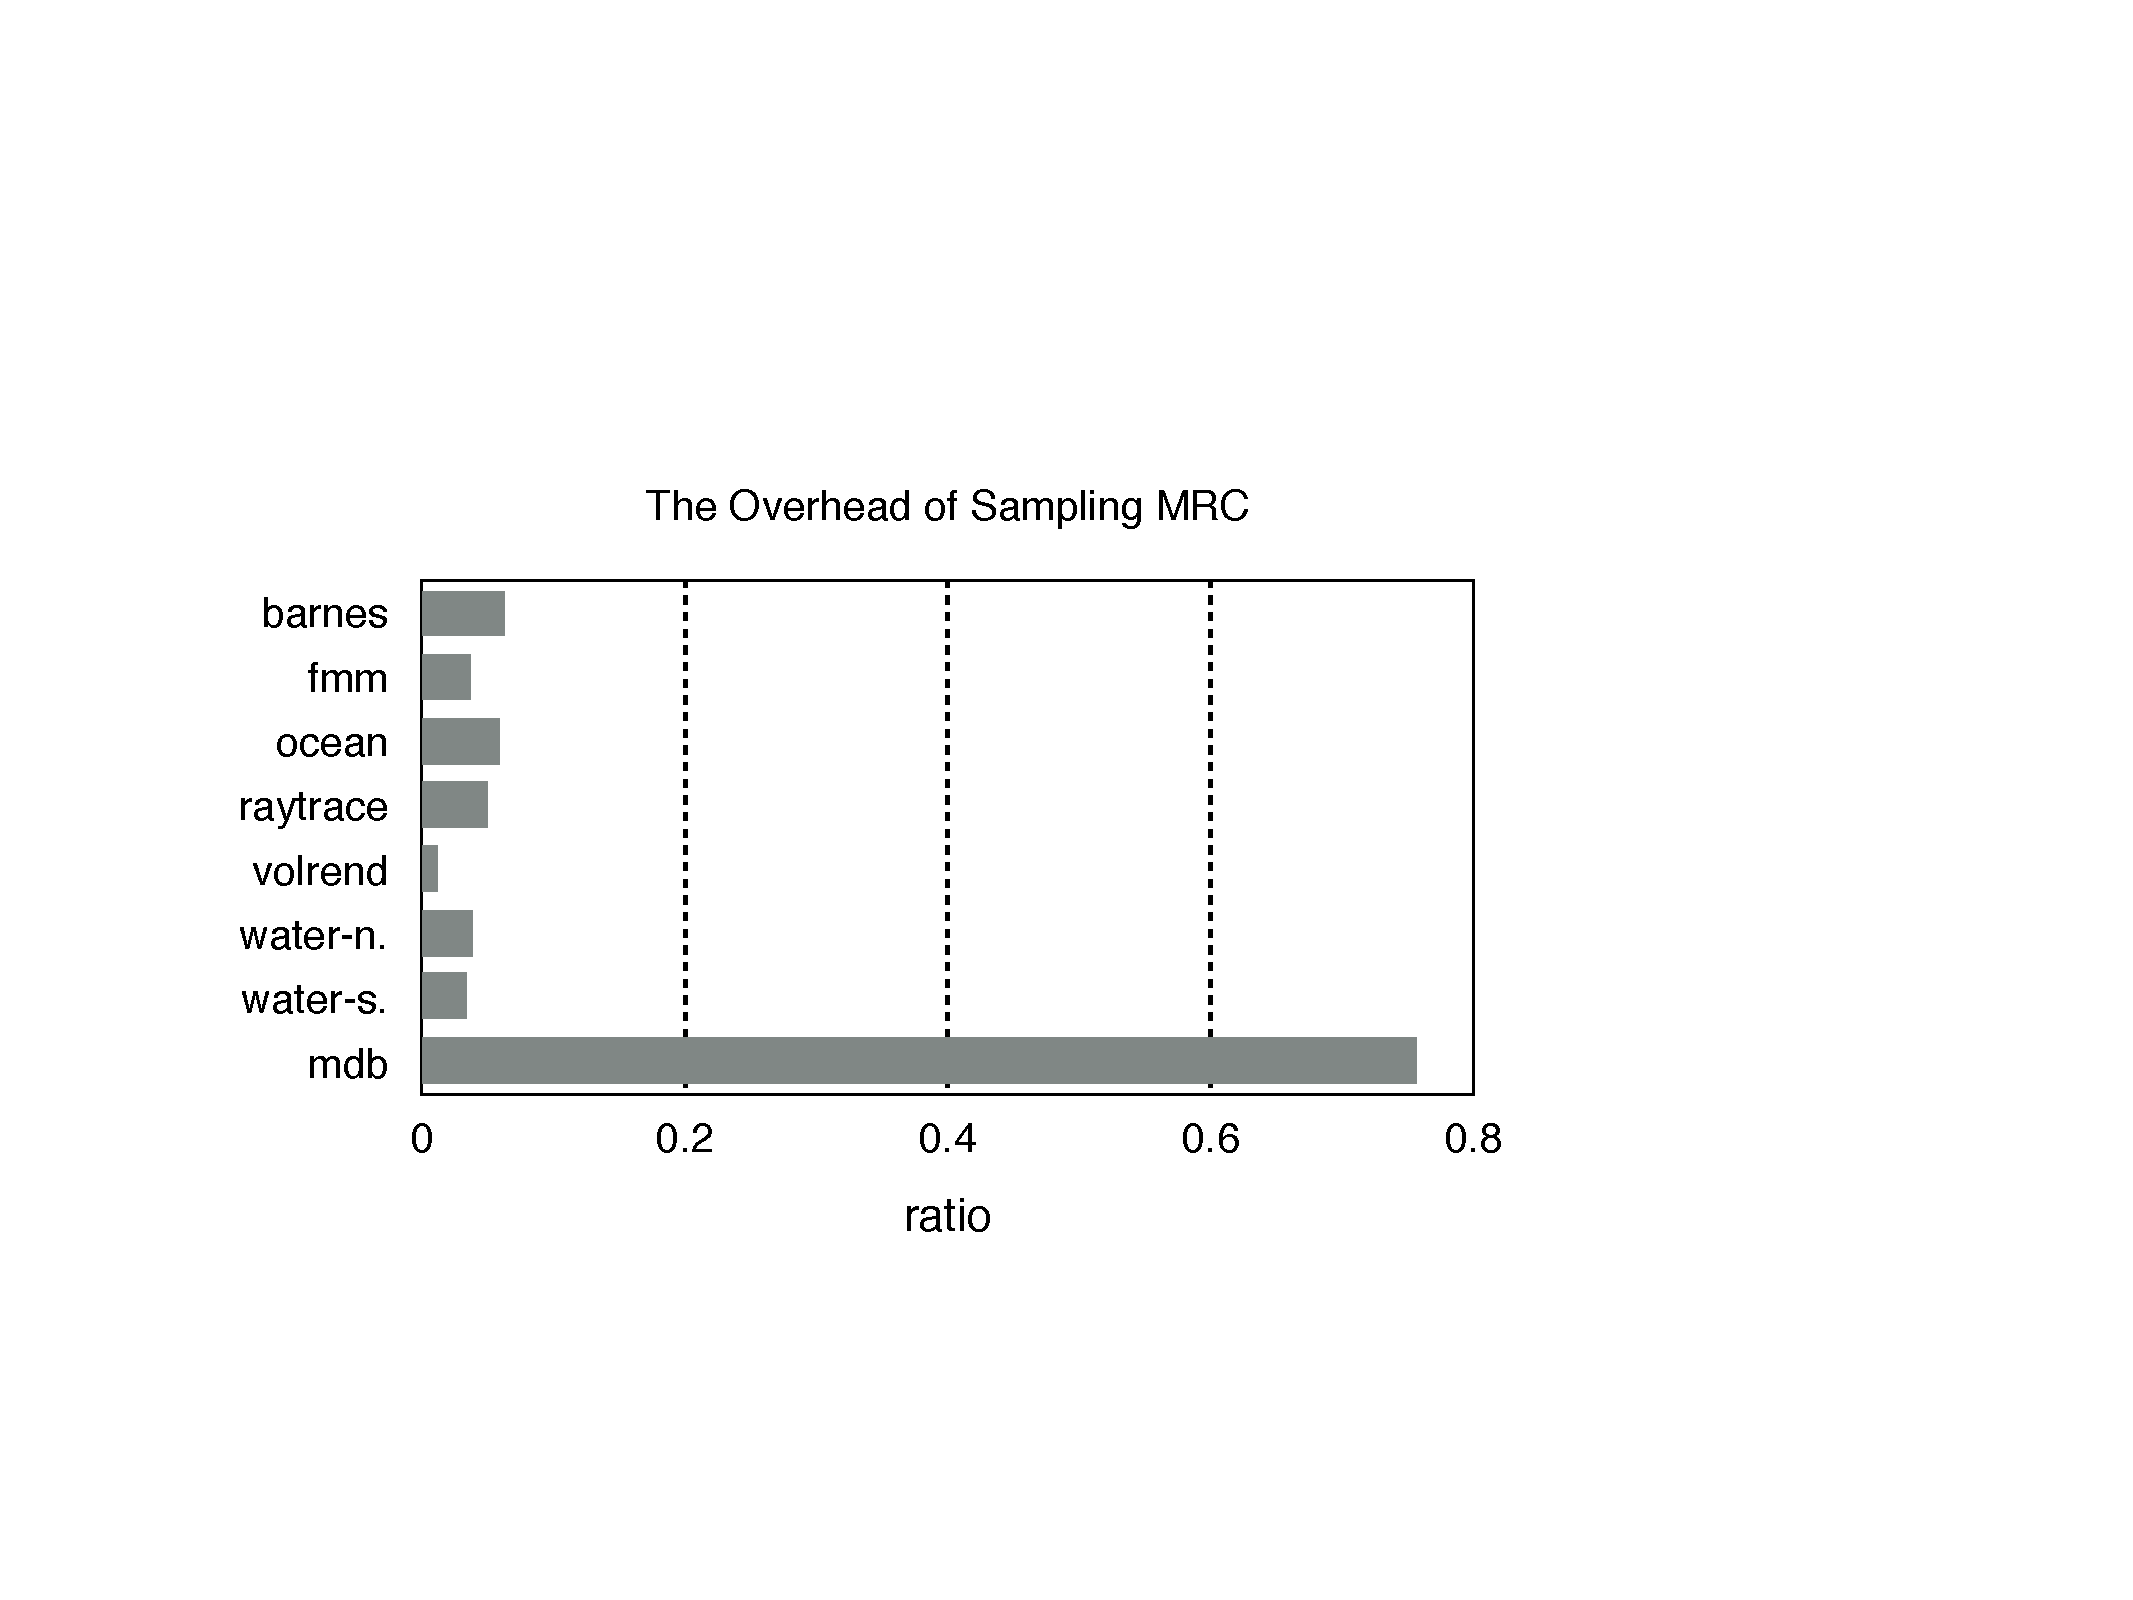
\includegraphics[width=8.5cm]{figures/mrc_overhead.pdf}
\caption{The running time ratio of sampling MRC. \emph{water-n.} denotes \emph{water-nsquared}.
 \emph{water-s.} denotes \emph{water-spatial}. }
\label{fig:mrc-ove}
\end{figure}

Figure~\ref{fig:model} shows that sampling MRC is effective to select the best
cache size. Figure~\ref{fig:mrc-ove} shows that the overhead of sampling MRC is 
very little. The average overhead of all programs but \emph{mdb} is 4\%. 
Adding it to the above performance data is just the performance of the software 
cache when calculating MRC online. It is still much better than the state-of-the-art AT.
\emph{Mdb}'s overhead is $75\%$. Since it runs shortly, the MRC overhead neglects 
performance gain. We believe that if \emph{mdb} runs like the cloud-end key-value 
store applications for days long, the overall program performance will be very optimistic, 
since the periodic selections of cache sizes benefit the program for a much longer execution. 
Therefore, we suggest that offline MRC-based optimization can be used for short-run 
programs to purse maximal performance, while the online MRC analysis is used for 
long-run applications, like the cloud-level applications.  


\section{Related Work}

\paragraph{Persistent memory programming}

\paragraph{MRC profiling}
Recent work[Wires et al. OSDI?14, Meng et al. ATC?14] starts to use
MRC curves to choose cache size. Results turn out that MRC is an effective
means. They use counter stacks[Wires et al. OSDI?14] or reuse distance
array[Meng et al. ATC?14] to construct MRC curves. In essence, they are
all variants of reuse distance[Ding and Zhong PLDI?03]. Reuse distance is
accurate, but costly to compute. The state-of-art work to compute it is
O(N(logM)) time, where N is the number of data accesses and M is the
number of distinct data accesses. To reduce time overhead, researchers often
prefer sampling to alleviate the computation.
In this work, we choose to use a window-based metric, called liveness[Li
et al. ISMM?14], to calculate MRC curves. Liveness-based calculation is
linear-time, which makes the MRC construction more practical.

\section{Summary}

%\bibliographystyle{abbrvnat}
\bibliographystyle{plain}
%\bibliography{references}
\bibliography{all}

\appendix

\section{MRCs of other programs}

\begin{figure}[hbpt]
\centering
\subfloat {
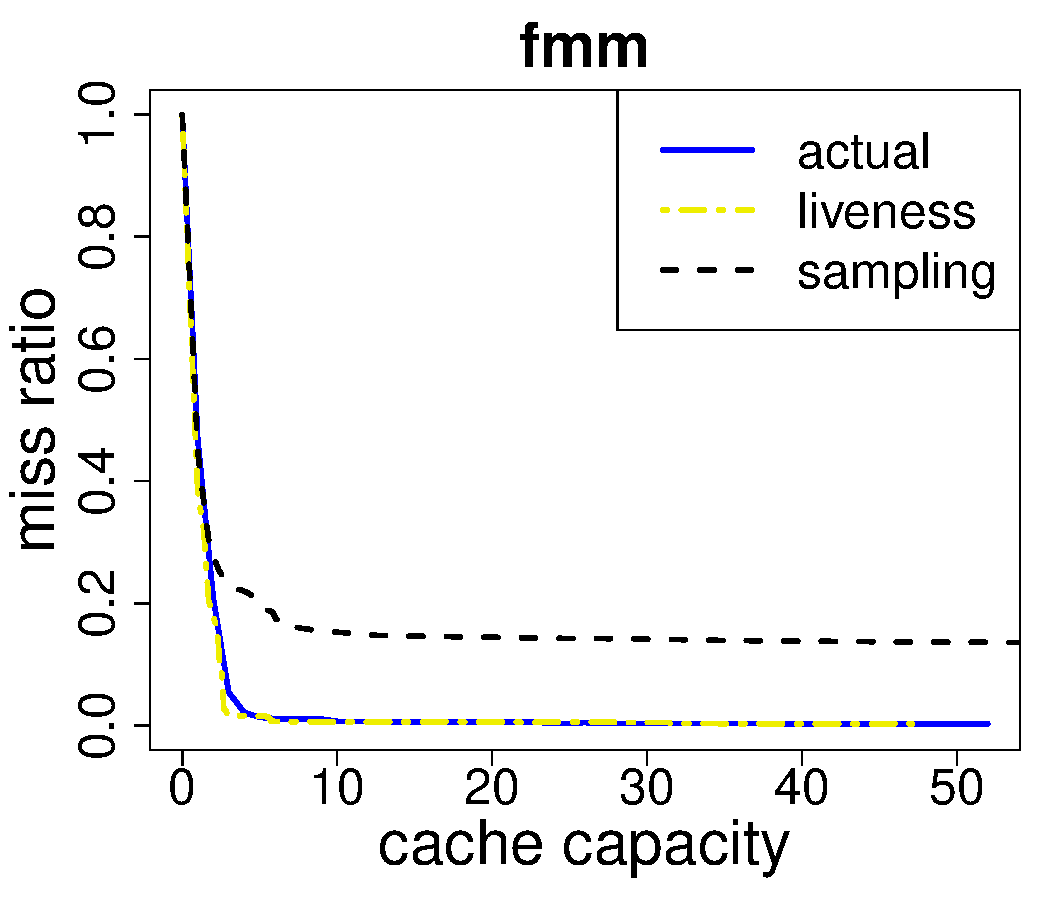
\includegraphics[width=4.3cm]{./figures/fmm.pdf}
\label{fig:simplutosolo}
}
\hspace*{-1em}
\subfloat {
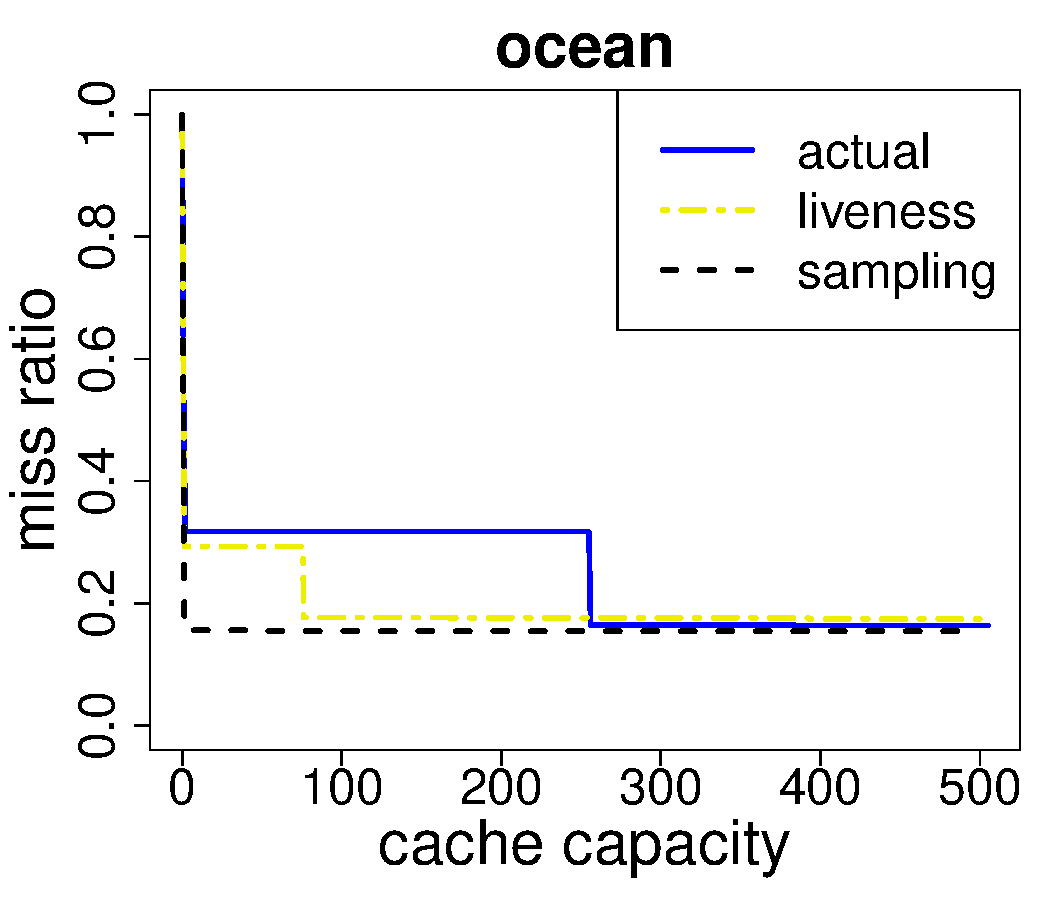
\includegraphics[width=4.3cm]{./figures/ocean_new.pdf}
\label{fig:simplutoco}
}
\vspace*{-1em}
\\
\subfloat {
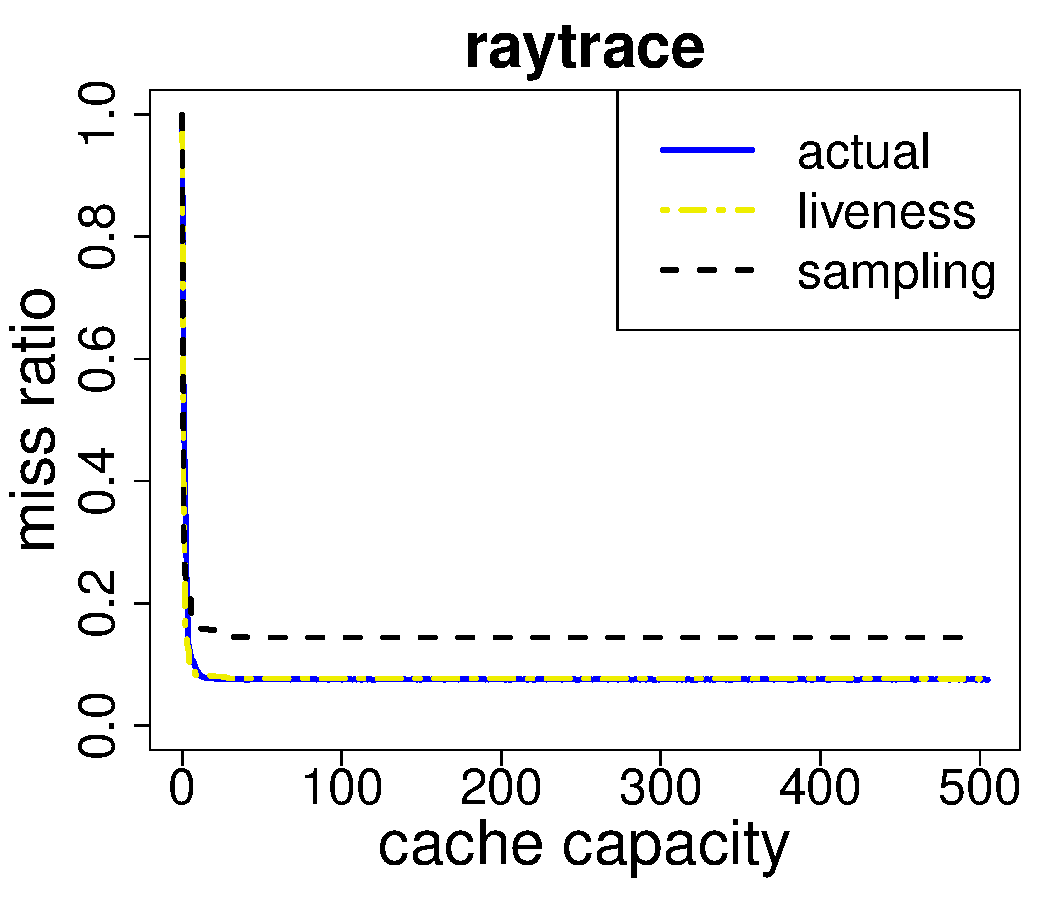
\includegraphics[width=4.3cm]{./figures/raytrace_new.pdf}
\label{fig:simplutosolo}
}
\hspace*{-1em}
\subfloat{
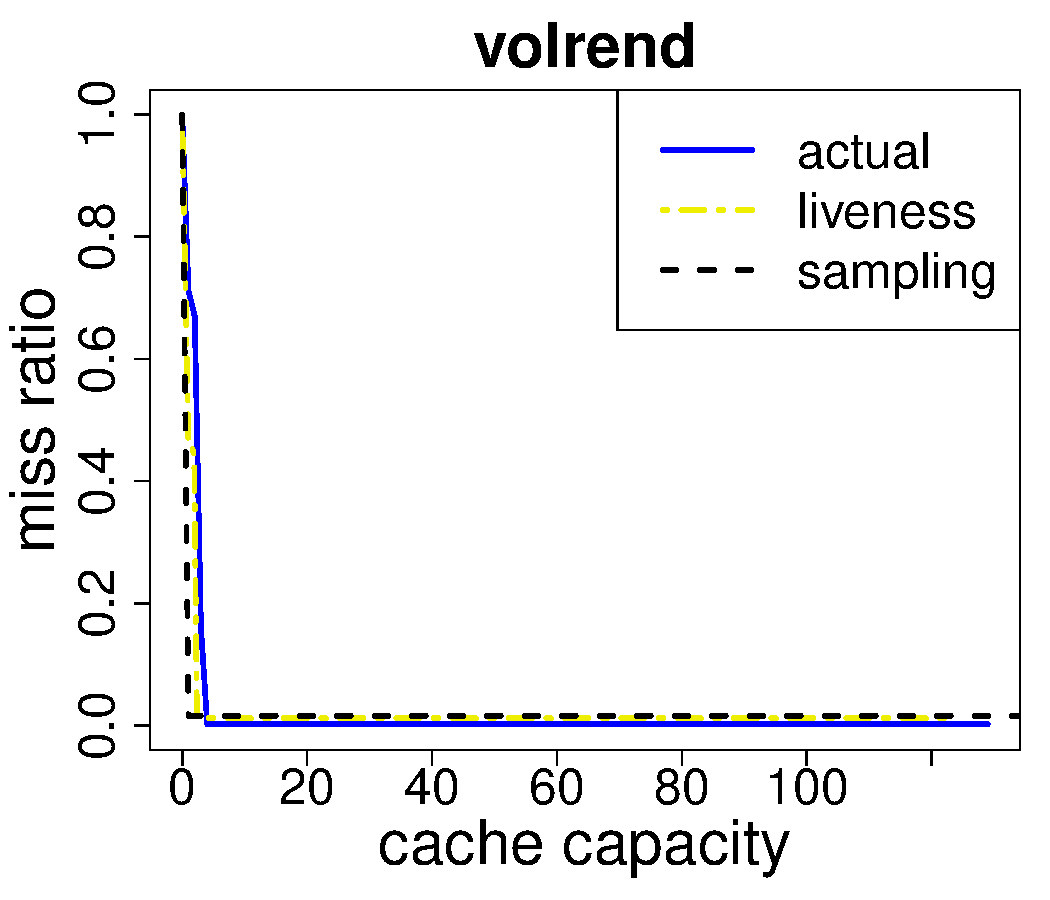
\includegraphics[width=4.3cm]{./figures/volrend_new.pdf}
\label{fig:simplutosolo}
}
\vspace*{-1em}
\\
\subfloat{
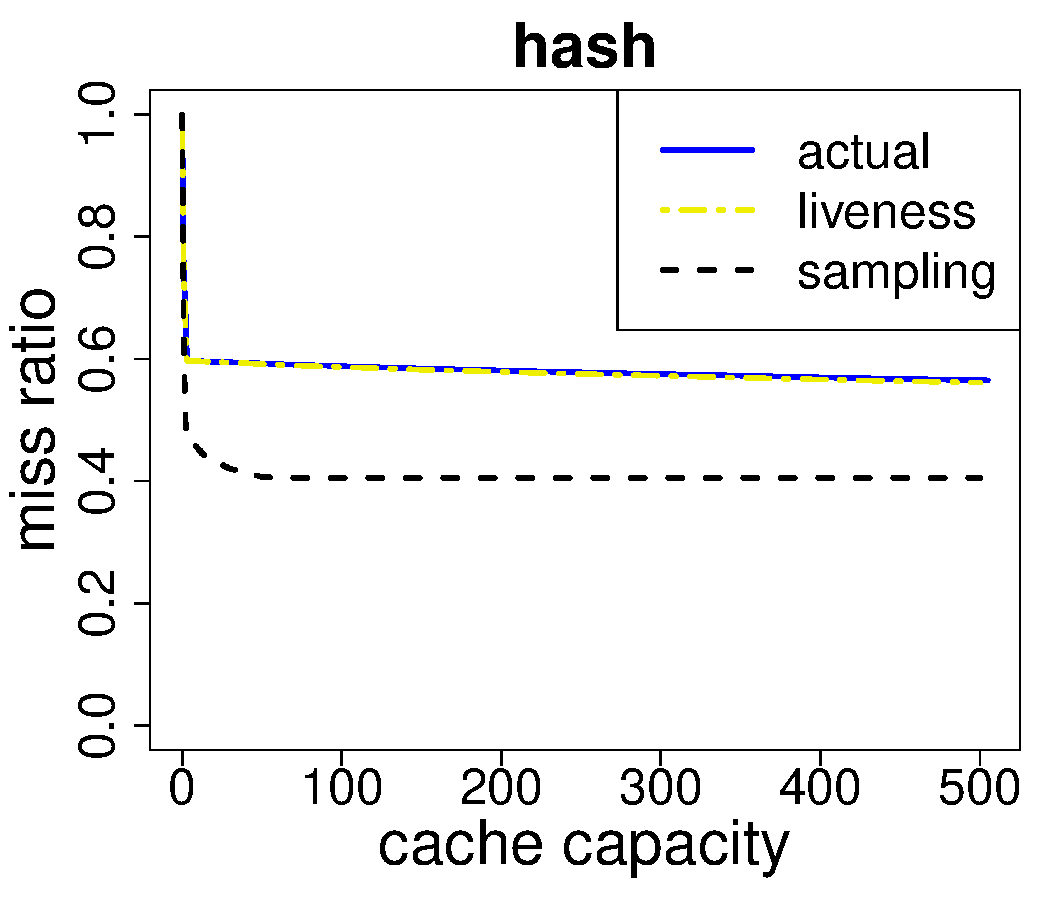
\includegraphics[width=4.3cm]{./figures/hash_new.pdf}
\label{fig:simplutosolo}
}
\hspace*{-1em}
\subfloat {
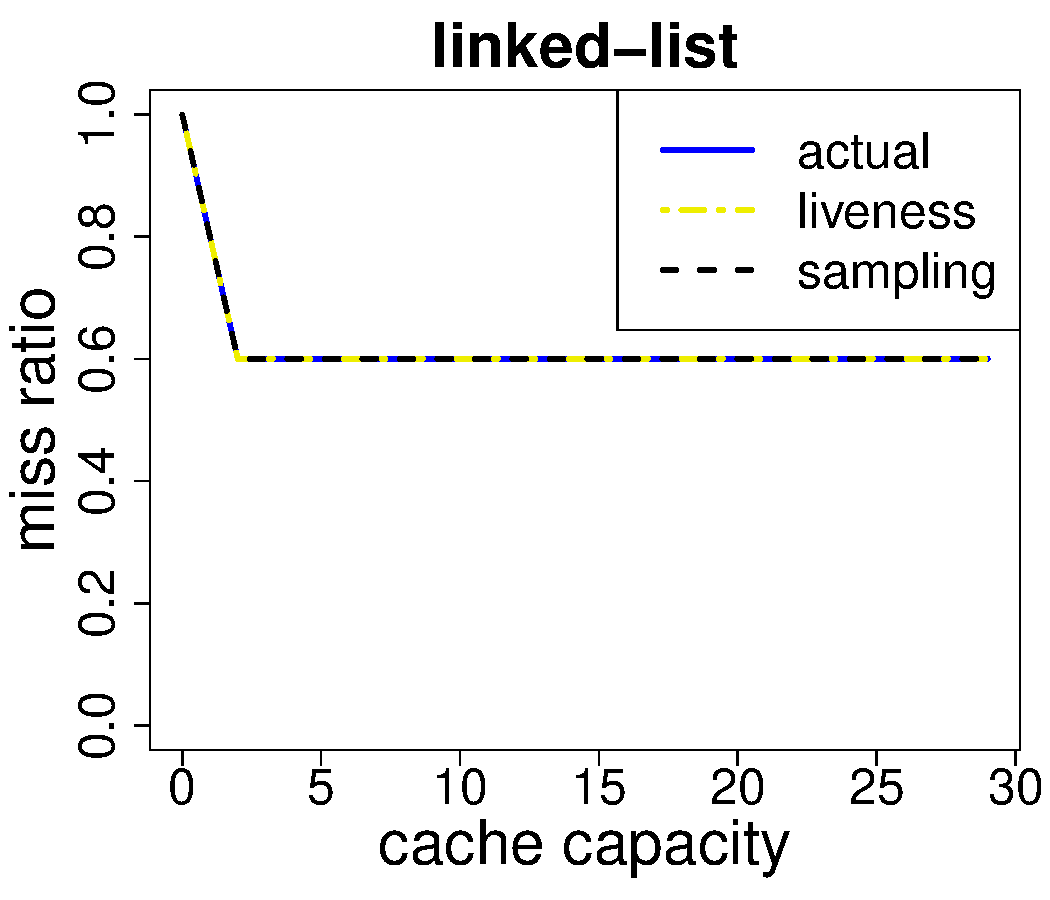
\includegraphics[width=4.3cm]{./figures/sll_new.pdf}
\label{fig:simplutoco}
}
\vspace*{-1em}
\\
\subfloat{
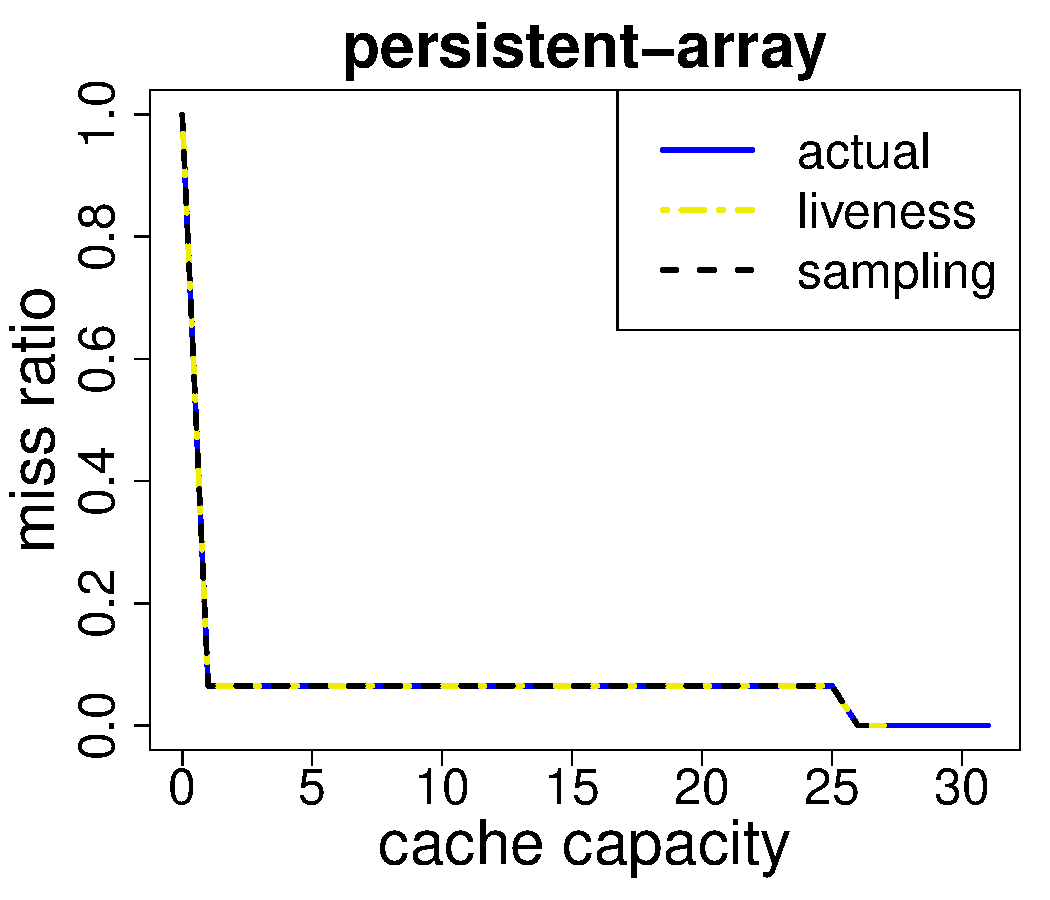
\includegraphics[width=4.3cm]{./figures/persis-array_new.pdf}
\label{fig:simplutosolo}
}
\hspace*{-1em}
\subfloat{
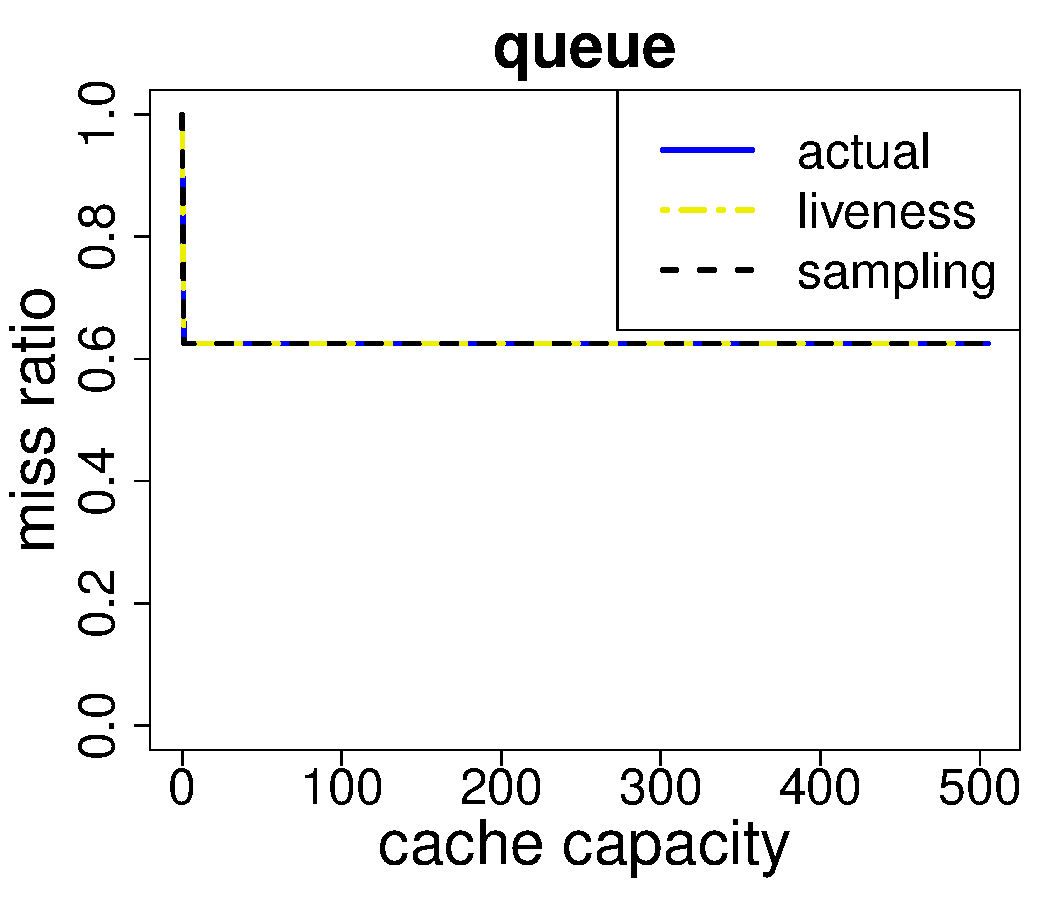
\includegraphics[width=4.3cm]{./figures/queue_new.pdf}
\label{fig:simplutosolo}
}
\caption{The comparison between actual MRC, accurate 
MRC and sampling modeled MRC of the other programs.}
\label{fig:model-appendix}
\end{figure}

\end{document}
